\subsection{\texorpdfstring{THE HOMOMORPHISM \(\mathbf{E}^* \otimes_{\mathbf{A}} \mathbf{F} \to \operatorname{Hom}_{\mathbf{A}}(\mathbf{E}, \mathbf{F})\)}{THE HOMOMORPHISM \textbackslash mathbf\{E\}\^{}* \textbackslash otimes\_\{\textbackslash mathbf\{A\}\} \textbackslash mathbf\{F\} \textbackslash to \textbackslash operatorname\{Hom\}\_\{\textbackslash mathbf\{A\}\}(\textbackslash mathbf\{E\}, \textbackslash mathbf\{F\})}}

Let A, B be two rings, E a left A-module, F a left B-module and G an (A, B)-bimodule. The Z-module \(\operatorname{Hom}_{\mathbf{A}}(\mathbf{E}, \mathbf{G})\) has canonically a right B-module structure (§ 1, no. 14) such that \((u\beta)(x) = u(x)\beta\) for \(\beta \in \mathbf{B}\) , \(u \in \operatorname{Hom}_{\mathbf{A}}(\mathbf{E}, \mathbf{G})\) , \(x \in \mathbf{E}\) . On the other hand, \(\mathbf{G} \otimes_{\mathbf{B}} \mathbf{F}\) has canonically a left A-module structure (§ 3, no. 4). We shall define a canonical \(\mathbf{Z}\) -homomorphism

\[
\nu : \operatorname{Hom} _ {\mathbf {A}} (\mathrm{E}, \mathrm{G}) \otimes_ {\mathbf {B}} \mathrm{F} \rightarrow \operatorname{Hom} _ {\mathbf {A}} (\mathrm{E}, \mathrm{G} \otimes_ {\mathbf {B}} \mathrm{F}).\tag{7}
\]

To this end, we consider, for all \(y \in \mathbf{F}\) and all \(u \in \operatorname{Hom}_{\mathbf{A}}(\mathbf{E}, \mathbf{G})\) , the mapping \(\nu'(u, y): x \mapsto u(x) \otimes y\) of \(\mathbf{E}\) onto \(\mathbf{G} \otimes_{\mathbf{B}} \mathbf{F}\) . It is immediately verified that \(\nu'(u, y)\) is A-linear and that \(\nu'\) is a Z-bilinear mapping of \(\operatorname{Hom}_{\mathbf{A}}(\mathbf{E}, \mathbf{G}) \times \mathbf{F}\) into \(\operatorname{Hom}_{\mathbf{A}}(\mathbf{E}, \mathbf{G} \otimes_{\mathbf{B}} \mathbf{F})\) ; moreover, for all \(\beta \in \mathbf{B}\) , \(\nu'(u\beta, y)\) and \(\nu'(u, \beta y)\) are equal, for \((u(x)\beta) \otimes y = u(x) \otimes (\beta y)\) . We conclude (§ 3, no. 1, Proposition 1) the existence of the desired homomorphism \(\nu\) such that \(\nu(u \otimes y)\) is the A-linear mapping \(x \mapsto u(x) \otimes y\) .

It is immediately verified that, if E is an \((\mathbf{A}, (\mathbf{C}_{i}^{\prime}) ; (\mathbf{D}_{j}^{\prime}))\) -multimodule, F a \((\mathbf{B}, (\mathbf{C}_{h}^{\prime\prime}) ; (\mathbf{D}_{k}^{\prime\prime}))\) -multimodule and G an \((\mathbf{A}, (\mathbf{C}_{l}^{\prime\prime}) ; \mathbf{B}, (\mathbf{D}_{m}^{\prime\prime}))\) -multimodule, the mapping (7) is a \(((\mathbf{D}_{j}^{\prime}), (\mathbf{C}_{h}^{\prime\prime}), (\mathbf{C}_{l}^{\prime\prime}) ; (\mathbf{C}_{i}^{\prime}), (\mathbf{D}_{k}^{\prime\prime}), (\mathbf{D}_{m}^{\prime\prime}))\) -multimodule homomorphism.

PROPOSITION 2. (i) When F is a projective (resp. finitely generated projective) B-module, the canonical homomorphism (7) is injective (resp. bijective).

\begin{enumerate}
\def\labelenumi{(\roman{enumi})}
\setcounter{enumi}{1}
\item
  When E is a finitely generated projective A-module, the canonical homomorphism (7) is bijective.
\item
  Fixing E and G, for every left B-module F, we write
\end{enumerate}

\[
\mathrm{T} (\mathrm{F}) = \operatorname{Hom} _ {\mathrm{A}} (\mathrm{E}, \mathrm{G}) \otimes_ {\mathrm{B}} \mathrm{F}, \quad \mathrm{T} ^ {\prime} (\mathrm{F}) = \operatorname{Hom} _ {\mathrm{A}} (\mathrm{E}, \mathrm{G} \otimes_ {\mathrm{B}} \mathrm{F});
\]

for every left B-module homomorphism \(u: \mathbf{F} \to \mathbf{F}'\) , we write \(\mathrm{T}(u) = 1 \otimes u\) (1 here denoting the identity mapping of \(\operatorname{Hom}_{\mathbf{A}}(\mathbf{E}, \mathbf{G})\) ),

\[
\mathrm{T} ^ {\prime} (u) = \operatorname{Hom} \left(\mathrm{l} _ {\mathbb {E}}, \mathrm{l} _ {\mathbb {G}} \otimes u\right);
\]

on the other hand we write \(\nu_{F}\) instead of \(\nu\). Then we have the following lemmas:

Lemma 1. For every homomorphism \(u: \mathbf{F} \to \mathbf{F}'\) , the diagram

\[
\begin{array}{c c c} \mathrm{T(F)} & \xrightarrow {\nu_ {\mathrm{F}}} & \mathrm {T^ {\prime} (F)} \\ \mathrm{T(u)} \Big \downarrow & & \Big \downarrow \mathrm {T^ {\prime} (u)} \\ \mathrm {T(F^ {\prime})} & \xrightarrow {\nu_ {\mathrm {F^ {\prime}}}} & \mathrm {T^ {\prime} (F^ {\prime})} \end{array}\tag{8}
\]

is commutative.

The verification is immediate.

Lemma 2. Let M, N be two supplementary submodules in F and i: M → F, j: N → F the canonical injections. The diagram

\begin{enumerate}
\def\labelenumi{(\arabic{enumi})}
\setcounter{enumi}{8}
\tightlist
\item
\end{enumerate}

\pandocbounded{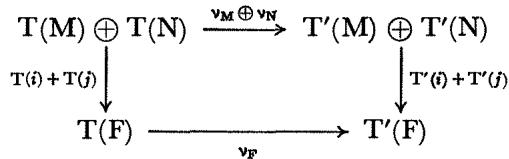
\includegraphics[keepaspectratio]{images/part002_2544dc0c.jpg}}

is commutative and the vertical arrows are bijective.

The commutativity follows from Lemma 1, the other assertions from § 1, no. 6, Corollary 2 to Proposition 6 and § 3, no. 7, Proposition 7.

Lemma 3. Under the hypotheses of Lemma 2, for \(\nu_{\mathrm{F}}\) to be injective (resp. surjective), it is necessary and sufficient that \(\nu_{\mathrm{M}}\) and \(\nu_{\mathrm{N}}\) be so.

This follows from Lemma 2 and § 1, no. 6, Corollary 1 to Proposition 6.

Then Lemma 3, together with §2, no. 2, Proposition 4, shows that it suffices to consider the case where F is a free module. But, if \((b_{\mu})\) is a basis of F, every element of \(\operatorname{Hom}_{\mathbf{A}}(\mathbf{E}, \mathbf{G}) \otimes_{\mathbf{B}} \mathbf{F}\) may then be written uniquely as \(\sum_{\mu} u_{\mu} \otimes b_{\mu}\) , where \(u_{\mu} \in \operatorname{Hom}_{\mathbf{A}}(\mathbf{E}, \mathbf{G})\) (§ 3, no. 7, Corollary 1 to Proposition 7); the image of this element under \(\nu\) is the A-linear mapping \(x \mapsto \sum_{\mu} u_{\mu}(x) \otimes b_{\mu}\) ; it cannot be zero for all \(x \in \mathbf{E}\) unless \(u_{\mu}(x) = 0\) for all \(x \in \mathbf{E}\) and all \(\mu\) , which is equivalent to saying that \(u_{\mu} = 0\) for all \(\mu\) ; hence \(\nu\) is injective. When also F admits a finite basis, Lemma 3 shows (by induction on the number of elements in the basis of F) that to prove that \(\nu\) is surjective, it suffices to do so when \(F = B_s\) ; but in this case the two sides of (7) are canonically identified with \(\operatorname{Hom}_{\mathbf{A}}(\mathbf{E}, \mathbf{G})\) (§ 3, no. 4, Proposition 4) and \(\nu\) becomes the identity.

\begin{enumerate}
\def\labelenumi{(\roman{enumi})}
\setcounter{enumi}{1}
\tightlist
\item
  To show the proposition when E is projective and finitely generated, this time we fix F and G and write, for every left A-module E,
\end{enumerate}

\[
\mathrm{T} (\mathrm{E}) = \operatorname{Hom} _ {\mathrm{A}} (\mathrm{E}, \mathrm{G}) \otimes_ {\mathrm{B}} \mathrm{F}, \quad \mathrm{T} ^ {\prime} (\mathrm{E}) = \operatorname{Hom} _ {\mathrm{A}} (\mathrm{E}, \mathrm{G} \otimes_ {\mathrm{B}} \mathrm{F})
\]

and, for every left A-module homomorphism \(v:\mathbf{E}\to\mathbf{E}^{\prime}\) ,

\[
\mathrm{T} (v) = \operatorname{Hom} (v, 1 _ {\mathbf {G}}) \otimes 1 _ {\mathbf {F}}, \quad \mathrm{T} ^ {\prime} (v) = \operatorname{Hom} (v, 1 _ {\mathbf {G}} \otimes 1 _ {\mathbf {F}});
\]

on the other hand, we write \(\nu_{E}\) instead of \(\nu\). Then we have the two lemmas:

Lemma 4. For every homomorphism \(v: \mathbf{E} \to \mathbf{E}'\) , the diagram

\[
\begin{array}{c c c} \mathrm{T} (\mathrm{E} ^ {\prime}) & \xrightarrow {\nu_ {\mathrm{E} ^ {\prime}}} & \mathrm{T} ^ {\prime} (\mathrm{E} ^ {\prime}) \\ \mathrm{T} (v) \Big \downarrow & & \Big \downarrow \mathrm{T} ^ {\prime} (v) \\ \mathrm{T} (\mathrm{E}) & \xrightarrow {\nu_ {\mathrm{E}}} & \mathrm{T} ^ {\prime} (\mathrm{E}) \end{array}\tag{10}
\]

is commutative.

Lemma 5. Let \(\mathbf{M}\) and \(\mathbf{N}\) be two supplementary submodules in \(\mathbf{E}\) and \(p: \mathbf{E} \to \mathbf{M}\) , \(q: \mathbf{E} \to \mathbf{N}\) the canonical projections. The diagram

\pandocbounded{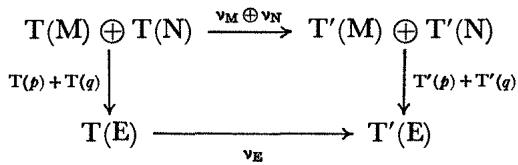
\includegraphics[keepaspectratio]{images/part002_a961576f.jpg}}

is commutative and the vertical arrows are bijective.

They are proved as Lemmas 1 and 2, taking account of § 1, no. 6, Corollary 2 to Proposition 6, § 2, no. 1, Proposition 1 and § 3, no. 7, Proposition 7.

The remainder of the proof then proceeds as in (i) and is reduced to the case where \(E = A_{s}\) ; the two sides of (7) are then canonically identified with \(G \otimes_{B} F\) and \(\nu\) becomes the identity.

In particular take B = A and G the (A, A)-bimodule \(_{s}A_{d}\) (§ 3, no. 4), so that the right A-module \(\operatorname{Hom}_{\mathbf{A}}(\mathbf{E}, _{s}\mathbf{A}_{d})\) is just the dual E* of E and \((_{s}\mathbf{A}_{d}) \otimes_{\mathbf{A}} F\) is canonically identified with F (§ 3, no. 4, Proposition 4). Homomorphism (7) then becomes a canonical Z-homomorphism

\[
\theta : \mathrm{E} ^ {*} \otimes_ {\mathrm{A}} \mathrm{F} \rightarrow \operatorname{Hom} _ {\mathrm{A}} (\mathrm{E}, \mathrm{F})\tag{11}
\]

and \(\theta (x^{*}\otimes y)\) is the linear mapping of E into F

\[
x \mapsto \langle x, x ^ {*} \rangle y.
\]

Remark (1). The characterization of projective A-modules given in §2, no. 6, Proposition 12, can also be expressed as follows: for a left A-module E to be projective, it is necessary and sufficient that the canonical homomorphism

\[
\theta_ {\mathbf {E}}: \mathrm{E} ^ {*} \otimes_ {\mathbf {A}} \mathrm{E} \rightarrow \operatorname{Hom} _ {\mathbf {A}} (\mathrm{E}, \mathrm{E}) = \operatorname{End} _ {\mathbf {A}} (\mathrm{E})
\]

be such that \(l_{E}\) belongs to the image of \(\theta_{E}\) .

COROLLARY. (i) When F is a projective (resp. finitely generated projective) module, the canonical homomorphism (11) is injective (resp. bijective).

\begin{enumerate}
\def\labelenumi{(\roman{enumi})}
\setcounter{enumi}{1}
\tightlist
\item
  When E is a finitely generated projective module, the canonical homomorphism (11) is bijective.
\end{enumerate}

Even when E and F are both finitely generated, \(\theta\) is not necessarily surjective, as is shown by the example A = Z, E = F = Z/2Z; the right hand side of (11) is non-zero but \(E^{*} = 0\) . On the other hand, examples can be given where E is free, but (11) is neither injective nor surjective (Exercise 3(b)).

When E admits a finite basis \((e_i)\) , the inverse isomorphism \(\theta^{-1}\) of \(\theta\) can be found explicitly as follows. Let \((e_i^*)\) be the dual basis of \((e_i)\) (§ 2, no. 6); for all \(u \in \operatorname{Hom}(\mathbf{E}, \mathbf{F})\) and all \(x = \sum_{i} \xi_i e_i\) with \(\xi_i \in \mathbf{A}\) ,

\[
u (x) = \sum_ {i} \xi_ {i} u (e _ {i}) = \sum_ {i} \langle x, e _ {i} ^ {*} \rangle u (e _ {i})
\]

and therefore \(u = \sum_{i} \theta(e_i^* \otimes u(e_i))\) , in other words

\[
\theta^ {- 1} (u) = \sum_ {i} e _ {i} ^ {*} \otimes u (e _ {i}).\tag{12}
\]

In particular, if further F = E, it is seen that the image under \(\theta_{E}^{-1}\) of the identity mapping \(l_{E}\) is the element \(\sum_{i} e_{i}^{*} \otimes e_{i}\) , which is therefore independent of the basis \((e_{i})\) considered in E.

Note on the other hand that when E is a finitely generated projective module the ring structure on \(\operatorname{End}_{\mathbf{A}}(\mathbf{E})\) can be transported by \(\theta_{E}^{-1}\) to \(E^{*}\otimes_{A}E\) ; it is immediately verified that, for x, y in E, \(x^{*}, y^{*}\) in \(E^{*}\) , in the ring \(\operatorname{End}_{\mathbf{A}}(\mathbf{E})\) ,

\[
\theta_ {\mathbf {E}} (x ^ {*} \otimes x) \circ \theta_ {\mathbf {E}} (y ^ {*} \otimes y) = \theta_ {\mathbf {E}} ((y ^ {*} \langle y, x ^ {*} \rangle) \otimes x).\tag{13}
\]

Remark (2). Let E be a right A-module; replacing E by E* in (11), we obtain a canonical Z-homomorphism

\[
\mathrm{E} ^ {* *} \otimes_ {\mathrm{A}} \mathrm{F} \rightarrow \operatorname{Hom} _ {\mathrm{A}} (\mathrm{E} ^ {*}, \mathrm{F}).\tag{14}
\]

On the other hand, there is a canonical A-homomorphism \(c_{E}:E\to E^{**}\) , whence there is a Z-homomorphism \(c_{E}\otimes l_{F}:E\otimes_{A}F\to E^{**}\otimes_{A}F\) ; composing the latter with the homomorphism (14), we hence obtain a canonical Z-homomorphism

\[
\theta^ {\prime}: \mathrm{E} \otimes_ {\mathrm{A}} \mathrm{F} \rightarrow \operatorname{Hom} _ {\mathrm{A}} (\mathrm{E} ^ {*}, \mathrm{F})\tag{15}
\]

such that \(\theta'(x \otimes y)\) is the linear mapping

\[
x ^ {*} \mapsto \langle x, x ^ {*} \rangle y.
\]

If E and F are projective modules, the mapping (15) is injective. For \(c_{E}\) is then injective (§2, no. 7, Corollary 4 to Proposition 13) and as F is projective, the Z-homomorphism \(c_{E} \otimes l_{F}: E \otimes_{A} F \to E^{**} \otimes_{A} F\) is also injective (§3, no. 7, Corollary 6 to Proposition 7); finally, it has been seen (Proposition 2) that the homomorphism (14) is injective, whence the conclusion.

If E is projective and finitely generated, the mapping (15) is bijective for the two mappings of which it is composed are then bijective (§ 2, no. 7, Corollary 4 to Proposition 13 and Proposition 2 above).

\subsection{TRACE OF AN ENDOMORPHISM}

Let C be a commutative ring and E a C-module. The mapping \((x^{*}, x) \mapsto \langle x, x^{*} \rangle\) of \(E^{*} \times E\) into C is then C-bilinear, since, for all \(\gamma \in C\) , \(\langle \gamma x, x^{*} \rangle = \gamma \langle x, x^{*} \rangle\) and \(\langle x, x^{*} \gamma \rangle = \langle x, x^{*} \rangle \gamma\) ; we derive a canonical C-linear mapping

\[
\tau : \mathbf {E} ^ {*} \otimes_ {\mathbf {c}} \mathbf {E} \rightarrow \mathbf {C}\tag{16}
\]

such that \(\tau(x^{*} \otimes x) = \langle x, x^{*} \rangle\) (§ 3, no. 5). Suppose now also that E is a finitely generated projective C-module; the canonical isomorphism (11) of no. 2 is then a C-module isomorphism and we can therefore define by transporting the structure a canonical linear form \(\mathrm{Tr} = \tau \circ \theta_{\mathbf{E}}^{-1}\) on the C-module \(\operatorname{End}_{\mathbf{C}}(\mathbf{E})\) . For all \(u \in \operatorname{End}_{\mathbf{C}}(\mathbf{E})\) the scalar \(\operatorname{Tr}(u)\) is called the trace of the endomorphism \(u\) ; every \(u \in \operatorname{End}_{\mathbf{C}}(\mathbf{E})\) can be written (in general in an infinity of ways) in the form \(x \mapsto \sum_{i} \langle x, x_{i}^{*} \rangle y_{i}\) where \(x_{i}^{*} \in \mathbf{E}^{*}\) and \(y_{i} \in \mathbf{E}_{i}\) by virtue of no. 2, Corollary to Proposition 2; then

\[
\operatorname{Tr} (u) = \sum_ {i} \left\langle y _ {i}, x _ {i} ^ {*} \right\rangle \quad (\text { cf. } \S 1 0, \text { no. } 1 1).\tag{17}
\]

By definition,

\begin{enumerate}
\def\labelenumi{(\arabic{enumi})}
\setcounter{enumi}{17}
\tightlist
\item
\end{enumerate}

\[
\operatorname{Tr} (u + v) = \operatorname{Tr} (u) + \operatorname{Tr} (v)\tag{19}
\]

\[
\operatorname{Tr} (\gamma u) = \gamma \operatorname{Tr} (u)
\]

for \(u, v\) in \(\operatorname{End}_{\mathbf{C}}(\mathbf{E})\) and \(\gamma \in \mathbf{C}\) . Moreover:

PROPOSITION 3. Let C be a commutative ring, E, F two finitely generated projective C-modules and \(u: \mathbf{E} \to \mathbf{F}\) and \(v: \mathbf{F} \to \mathbf{E}\) two linear mappings; then

\[
\operatorname{Tr} (v \circ u) = \operatorname{Tr} (u \circ v).\tag{20}
\]

The two mappings \((u, v) \mapsto \operatorname{Tr}(u \circ v)\) , \((u, v) \mapsto \operatorname{Tr}(v \circ u)\) of

\[
\operatorname{Hom} _ {\mathbf {c}} (\mathbf {E}, \mathbf {F}) \times \operatorname{Hom} _ {\mathbf {c}} (\mathbf {F}, \mathbf {E})
\]

into C are C-bilinear; it therefore suffices to verify (20) when u is of the form \(x \mapsto \langle x, a^{*} \rangle b\) and v of the form \(y \mapsto \langle y, b^{*} \rangle a\) , with \(a \in E\) , \(a^{*} \in E^{*}\) , \(b \in F\) , \(b^{*} \in F^{*}\) . But then \(v \circ u\) is the mapping \(x \mapsto \langle x, a^{*} \rangle \langle b, b^{*} \rangle a\) and \(u \circ v\) the mapping \(y \mapsto \langle y, b^{*} \rangle \langle a, a^{*} \rangle b\) . Formula (17) shows that the values of the two sides of (20) are equal to \(\langle a, a^{*} \rangle \langle b, b^{*} \rangle\) .

COROLLARY. If \(u_1, \ldots, u_p\) are endomorphisms of \(\mathbf{E}\) , then

\[
\operatorname{Tr} \left(u _ {1} \circ u _ {2} \circ \dots \circ u _ {p}\right) = \operatorname{Tr} \left(u _ {i} \circ u _ {i + 1} \circ \dots \circ u _ {p} \circ u _ {1} \circ \dots \circ u _ {i - 1}\right)
\]

for \(1 \leqslant i \leqslant p\) (``invariance of the trace under cyclic permutation'').

It suffices to apply (20) to the product

\[
\left(u _ {1} \circ u _ {2} \circ \dots \circ u _ {i - 1}\right) \circ \left(u _ {i} \circ u _ {i + 1} \circ \dots \circ u _ {p}\right).
\]

Note that on the other hand it is not necessarily true that

\[
\operatorname{Tr} (u \circ v \circ w) = \operatorname{Tr} (u \circ w \circ v)
\]

for three endomorphisms u, v, w of E.

\subsection{\texorpdfstring{THE HOMOMORPHISM \(\operatorname{Hom}_{\mathbb{C}}(\mathrm{E}_1, \mathrm{F}_1) \otimes_{\mathbb{C}} \operatorname{Hom}_{\mathbb{C}}(\mathrm{E}_2, \mathrm{F}_2) \to \operatorname{Hom}_{\mathbb{C}}(\mathrm{E}_1 \otimes_{\mathbb{C}} \mathrm{E}_2, \mathrm{F}_1 \otimes_{\mathbb{C}} \mathrm{F}_2)\)}{The homomorphism from Hom over C of E1,F1 tensor Hom over C of E2,F2 to Hom over C of the corresponding tensor products}}

Let C be a commutative ring and \(E_{1}\) , \(E_{2}\) , \(F_{1}\) , \(F_{2}\) four C-modules; in §3, no. 5, formula (13) we defined a canonical C-module homomorphism

\[
\lambda : \operatorname{Hom} (\mathbf {E} _ {1}, \mathbf {F} _ {1}) \otimes \operatorname{Hom} (\mathbf {E} _ {2}, \mathbf {F} _ {2}) \to \operatorname{Hom} (\mathbf {E} _ {1} \otimes \mathbf {E} _ {2}, \mathbf {F} _ {1} \otimes \mathbf {F} _ {2}). \tag {21}
\]

PROPOSITION 4. When one of the ordered pairs \((\mathbf{E}_1, \mathbf{E}_2)\) , \((\mathbf{E}_1, \mathbf{F}_1)\) , \((\mathbf{E}_2, \mathbf{F}_2)\) consists of finitely generated projective C-modules, the canonical homomorphism (21) is bijective.

It is obviously sufficient to perform the proof for the ordered pairs \((\mathbf{E}_{1}, \mathbf{F}_{1})\) and \((\mathbf{E}_{1}, \mathbf{E}_{2})\) .

We consider first the case of the ordered pair \((\mathbf{E}_1, \mathbf{F}_1)\) ; we fix \(\mathbf{E}_2, \mathbf{F}_1, \mathbf{F}_2\) and write for every C-module \(\mathrm{T}(\mathbf{E}) = \mathrm{Hom}(\mathbf{E}, \mathbf{F}_1) \otimes_{\mathbb{C}} \mathrm{Hom}(\mathbf{E}_2, \mathbf{F}_2)\) and \(\mathrm{T}'(\mathbf{E}) = \mathrm{Hom}(\mathbf{E} \otimes \mathbf{E}_2, \mathbf{F}_1 \otimes \mathbf{F}_2)\) and, for every C-homomorphism \(v: \mathbf{E} \to \mathbf{E}'\) ,

\[
\mathrm{T} (v) = \operatorname{Hom} (v, \mathrm{l} _ {\mathrm{F} _ {1}}) \otimes \mathrm{l} _ {\operatorname{Hom} (\mathrm{E} _ {2}, \mathrm{F} _ {2})}
\]

and

\[
\mathrm{T} ^ {\prime} (v) = \operatorname{Hom} (v \otimes 1 _ {\mathbb {E} _ {2}}, 1 _ {\mathbf {F} _ {1} \otimes \mathbf {F} _ {2}}).
\]

Then Lemmas 4 and 5 (no. 2) (where v is replaced by λ) are valid and are proved by completely analogous methods.

We next fix \(\mathbf{E}_2\) and \(\mathbf{F}_2\) and this time write, for every C-module \(\mathbf{F}\) , \(\mathrm{T}(\mathbf{F}) = \mathrm{Hom}(\mathbf{C},\mathbf{F})\otimes_{\mathbb{C}}\mathrm{Hom}(\mathbf{E}_2,\mathbf{F}_2)\) and \(\mathrm{T}'(\mathrm{F}) = \mathrm{Hom}(\mathbf{C}\otimes \mathbf{E}_2,\mathbf{F}\otimes \mathbf{F}_2)\) and, for every C-homomorphism \(u:\mathrm{F}\to \mathrm{F}'\) ,

\[
\mathrm{T} (u) = \operatorname{Hom} (\mathrm{l} _ {\mathbf {c}}, u) \otimes \mathrm{l} _ {\operatorname{Hom} (\mathbb {E} _ {2}, \mathrm{F} _ {2})}
\]

and

\[
\mathrm{T} ^ {\prime} (u) = \operatorname{Hom} (\mathrm{l} _ {\mathrm{c}} \otimes \mathrm{l} _ {\mathrm{E} _ {2}}, u \otimes \mathrm{l} _ {\mathrm{F} _ {2}}).
\]

This time it is immediately verified that Lemmas 1 and 2 (no. 2) (where \(\lambda\) always replaces \(\nu\) ) are valid.

This being so, we show the proposition first when \(E_{1} = C\) and \(F_{1}\) is projective and finitely generated. The argument of no. 2 (which rests on Lemmas 1 and 2), together with the above remarks, reduces this to proving the proposition when also \(F_{1} = C\) ; then \(\operatorname{Hom}(E_{1}, F_{1})\) , \(E_{1} \otimes E_{2}\) and \(F_{1} \otimes F_{2}\) are identified with C, \(E_{2}\) and \(F_{2}\) respectively (§ 3, no. 4, Proposition 4); the two sides of (21) are then both canonically identified with \(\operatorname{Hom}(\mathbf{E}_{2},\mathbf{F}_{2})\) and, after these identifications, it is verified that \(\lambda\) becomes the identity.

We now suppose that \(F_{1}\) is projective and finitely generated; the argument of no. 2 (depending this time on Lemmas 4 and 5) reduces the proof for \(E_{1}\) any finitely generated projective module to the case where \(E_{1} = C\) , that is to the first case dealt with.

For the ordered pair \((\mathbf{E}_{1}, \mathbf{E}_{2})\) , the procedure is similar, this time applying Lemmas 4 and 5 twice; we leave the details to the reader.

Note that when \(\mathbf{E}_1 = \mathbf{C}^{(I)}\) , \(\mathbf{E}_2 = \mathbf{C}^{(J)}\) are free (finitely generated or not), then \(\operatorname{Hom}(\mathbf{E}_1, \mathbf{F}_1) = \mathbf{F}_1^{\mathrm{I}}\) , \(\operatorname{Hom}(\mathbf{E}_2, \mathbf{F}_2 = \mathbf{F}_2^{\mathrm{J}}\) and

\[
\operatorname{Hom} \left(\mathrm{E} _ {1} \otimes \mathrm{E} _ {2}, \mathrm{F} _ {1} \otimes \mathrm{F} _ {2}\right) = \left(\mathrm{F} _ {1} \otimes \mathrm{F} _ {2}\right) ^ {\mathrm{I} \times \mathrm{J}}
\]

to within canonical isomorphisms and (21) is then identical with a special case of the canonical homomorphism (22) of § 3, no. 7.

When \(E_{2} = C\) , the canonical homomorphism (21) gives, after identifying \(\operatorname{Hom}(E_{2}, F_{2})\) with \(F_{2}\) and \(E_{1} \otimes E_{2}\) with \(E_{1}\) , a canonical homomorphism

\[
\operatorname{Hom} (\mathrm{E}, \mathrm{F}) \otimes \mathrm{G} \rightarrow \operatorname{Hom} (\mathrm{E}, \mathrm{F} \otimes \mathrm{G})\tag{22}
\]

for any three C-modules E, F, G which is just the homomorphism (7) of no. 2 for \(\mathbf{A} = \mathbf{B} = \mathbf{C}\) .

Note that when \(\mathbf{F} = \mathbf{C}\) the canonical homomorphism (22) again gives (11) (no. 2) for the case of a commutative ring.

Suppose now that \(\mathbf{F}_1 = \mathbf{F}_2 = \mathbf{C}\) ; as \(\mathbf{F}_1 \otimes \mathbf{F}_2\) is identified with \(\mathbf{C}\) , there is this time a canonical homomorphism

\[
\mu : \mathbf {E} ^ {*} \otimes \mathbf {F} ^ {*} \rightarrow (\mathbf {E} \otimes \mathbf {F}) ^ {*}\tag{23}
\]

for two C-modules E, F; for \(x^{*} \in \mathbf{E}^{*}\) , \(y^{*} \in \mathbf{F}^{*}\) , the image of \(x^{*} \otimes y^{*}\) under the canonical homomorphism (23) is the linear form \(u\) on \(\mathbf{E} \otimes \mathbf{F}\) such that

\[
u (x \otimes y) = \langle x, x ^ {*} \rangle \langle y, y ^ {*} \rangle .\tag{24}
\]

Moreover, if \(E_{1}\) , \(E_{2}\) , \(F_{1}\) , \(F_{2}\) are four C-modules, \(f: E_{1} \rightarrow E_{2}\) , \(g: F_{1} \rightarrow F_{2}\) two linear mappings, it follows immediately from (24) that the diagram

\[
\begin{array}{c} \mathrm{E} _ {2} ^ {*} \otimes \mathrm{F} _ {2} ^ {*} \xrightarrow {\mu} (\mathrm{E} _ {2} \otimes \mathrm{F} _ {2}) ^ {*} \\ t _ {f} \otimes t _ {g} \Biggl \downarrow \qquad \qquad \qquad \qquad \qquad \qquad \qquad \qquad \qquad \qquad \qquad \qquad \qquad \qquad \qquad \qquad \qquad \qquad \qquad \qquad \qquad \qquad \qquad \qquad \qquad \qquad \qquad \qquad \qquad \qquad \qquad \qquad \qquad \qquad \\ \mathrm{E} _ {1} ^ {*} \otimes \mathrm{F} _ {1} ^ {*} \xrightarrow {\mu} (\mathrm{E} _ {1} \otimes \mathrm{F} _ {1}) ^ {*} \end{array}\tag{25}
\]

is commutative.

COROLLARY 1. If one of the modules E, F is projective and finitely generated, the canonical homomorphism (23) is bijective.

COROLLARY 2. Let \(\mathbf{E}_1, \mathbf{E}_2\) be two finitely generated projective C-modules, \(u_1\) an endomorphism of \(\mathbf{E}_1\) and \(u_2\) an endomorphism of \(\mathbf{E}_2\) ; then

\[
\operatorname{Tr} (u _ {1} \otimes u _ {2}) = \operatorname{Tr} (u _ {1}) \operatorname{Tr} (u _ {2}).\tag{26}
\]

By linearity, it suffices to consider the case where \(u_{1}\) is of the form \(x_{1} \mapsto \langle x_{1}, x_{1}^{*} \rangle y_{1}\) and \(u_{2}\) of the form \(x_{2} \mapsto \langle x_{2}, x_{2}^{*} \rangle y_{2}\) ; then the image of \(x_{1} \otimes x_{2}\) under \(u_{1} \otimes u_{2}\) is by definition

\[
\langle x _ {1}, x _ {1} ^ {*} \rangle \langle x _ {2}, x _ {2} ^ {*} \rangle (y _ {1} \otimes y _ {2}) = \langle x _ {1} \otimes x _ {2}, x _ {1} ^ {*} \otimes x _ {2} ^ {*} \rangle (y _ {1} \otimes y _ {2})
\]

\(x_{1}^{*}\otimes x_{2}^{*}\) being canonically identified under \(\mu\) with an element of \((\mathrm{E}_{1}\otimes\mathrm{E}_{2})^{*}\) . As \(\langle y_{1}\otimes y_{2},x_{1}^{*}\otimes x_{2}^{*}\rangle=\langle y_{1},x_{1}^{*}\rangle\langle y_{2},x_{2}^{*}\rangle\) , formula (26) follows in this case from (17).

Remark. If E, F, G are any three C-modules, it is immediately verified that the diagram

\[
\begin{array}{c} \mathrm{E} ^ {*} \otimes \mathrm{F} ^ {*} \otimes \mathrm{G} ^ {*} \xrightarrow {\mu \otimes 1} (\mathrm{E} \otimes \mathrm{F}) ^ {*} \otimes \mathrm{G} ^ {*} \\ 1 \otimes \mu \Biggl \downarrow \\ \mathrm{E} ^ {*} \otimes (\mathrm{F} \otimes \mathrm{G}) ^ {*} \xrightarrow [ \mu ]{} (\mathrm{E} \otimes \mathrm{F} \otimes \mathrm{G}) ^ {*} \end{array}\tag{27}
\]

is commutative, by virtue of formula (24).

We note also that, without any hypothesis on the C-modules E, F, there are canonical isomorphisms

\begin{enumerate}
\def\labelenumi{(\arabic{enumi})}
\setcounter{enumi}{27}
\tightlist
\item
\end{enumerate}

\[
(\mathbf {E} \otimes \mathbf {F}) ^ {*} \rightarrow \operatorname{Hom} (\mathbf {E}, \mathbf {F} ^ {*})\tag{29}
\]

\[
(\mathbf {E} \otimes \mathbf {F}) ^ {*} \rightarrow \operatorname{Hom} (\mathbf {F}, \mathbf {E} ^ {*})
\]

which are just the isomorphism (6) and (5) of no. 1 for \(\mathbf{G} = \mathbf{C}\) , \(\mathbf{A} = \mathbf{B} = \mathbf{C}\) .

Thus a canonical one-to-one correspondence has been defined between the bilinear forms on \(E \times F\) , the homomorphisms of E into \(F^{*}\) and the homomorphisms of F into \(E^{*}\) : if u (resp. v) is a homomorphism of E into \(F^{*}\) (resp. of F into \(E^{*}\) ), the corresponding bilinear form is given by

\[
(x, y) \mapsto \langle y, u (x) \rangle \quad (\text { resp. } (x, y) \mapsto \langle x, v (y) \rangle).
\]

\section{EXTENSION OF THE RING OF SCALARS}

\subsection{EXTENSION OF THE RING OF SCALARS OF A MODULE}

Let A, B be two rings and \(\rho: \mathbf{A} \to \mathbf{B}\) a ring homomorphism; we consider the right A-module \(\rho^{*}(B_{d})\) defined by this homomorphism (§ 1, no. 13); this A-module also has a left B-module structure, namely that of \(B_{s}\) and, as \(b'(b\rho(a)) = (b'b)\rho(a)\) for \(a \in \mathbf{A}\) , \(b\) , \(b'\) in B, these two module structures on B are compatible (§ 1, no. 14). This allows us, for every left A-module E, to define a left B-module structure on the tensor product \(\rho_{*}(B_{d}) \otimes_{\mathbf{A}} \mathbf{E}\) such that \(\beta'(\beta \otimes x) = (\beta'\beta) \otimes x\) for \(\beta\) , \(\beta'\) in B and \(x \in \mathbf{E}\) (§ 3, no. 3). This left B-module is said to be derived from E by extending the ring of scalars to B by means of \(\rho\) and it is denoted by \(\rho^{*}(\mathbf{E})\) or \(\mathrm{E}_{(\mathbf{B})}\) if no confusion arises.

PROPOSITION 1. For every left A-module E, the mapping \(\phi: x \mapsto 1 \otimes x\) of E into the A-module \(\rho_*(\rho^*(\mathbf{E}))\) is A-linear and the set \(\phi(\mathbf{E})\) generates the B-module \(\rho^*(\mathbf{E})\) . Further, for every left B-module F and every A-linear mapping \(f\) of E into the A-module \(\rho_*(\mathbf{F})\) , there exists one and only one B-linear mapping \(\tilde{f}\) of \(\rho^*(\mathbf{E})\) into F such that \(\tilde{f}(1 \otimes x) = f(x)\) for all \(x \in \mathbf{E}\) .

B can be considered as a (B, A)-bimodule by means of \(\rho\) ; then there is a canonical Z-module isomorphism

\[
\operatorname{Hom} _ {\mathbf {B}} (\mathbf {B} \otimes_ {\mathbf {A}} \mathbf {E}, \mathbf {F}) \rightarrow \operatorname{Hom} _ {\mathbf {A}} (\mathbf {E}, \operatorname{Hom} _ {\mathbf {B}} (\mathbf {B} _ {s}, \mathbf {F}))\tag{1}
\]

as has been seen in § 4, no. 1, Proposition 1. But the left A-module \(\mathrm{Hom}_{\mathbf{B}}(\mathbf{B}_{s},\mathbf{F})\) is canonically identified with \(\rho^{*}(\mathbf{F})\) : for, by definition (§ 1, no. 14), there corresponds to an element \(y\in \mathbf{F}\) the homomorphism \(\theta (y)\colon \mathbf{B}_s\to \mathbf{F}\) such that \((\theta (y))(1) = y\) ; for all \(\lambda \in \mathbf{A}\) , there thus corresponds to \(\rho (\lambda)y\in \mathbf{F}\) the homomorphism \(\mu \mapsto \mu \rho (\lambda)y\) of \(\mathbf{B}_s\) into \(\mathbf{F}\) , which is just \(\lambda \theta (y)\) for the left A-module structure on \(\mathrm{Hom}_{\mathbf{B}}(\mathbf{B}_{s},\mathbf{F})\) (§ 1, no. 14). Using this identification, we obtain therefore a canonical Z-module isomorphism, the inverse of (1)

\[
\delta : \operatorname{Hom} _ {\mathbf {A}} (\mathbf {E}, \rho_ {*} (\mathbf {F})) \rightarrow \operatorname{Hom} _ {\mathbf {B}} (\rho^ {*} (\mathbf {E}), \mathbf {F})\tag{2}
\]

and it follows immediately from the definitions that if \(\delta(f) = \bar{f}\) then \(\bar{f}(1 \otimes x) = f(x)\) for all \(x \in \mathbf{E}\) . In particular, the mapping \(\phi_{\mathbb{E}}: x \mapsto 1 \otimes x\) is just

\[
\phi_ {\mathbf {E}} = \delta^ {- 1} (1 _ {\rho^ {*} (\mathbf {E})}).\tag{3}
\]

Proposition 1 is therefore proved. The mapping \(\phi_{\mathbf{E}}: \mathbf{E} \to \rho_{*}(\rho^{*}(\mathbf{E}))\) is called canonical.

Remarks. (1) Proposition 1 shows that the ordered pair consisting of \(\mathbf{E}_{(\mathbf{B})}\) and \(\phi_{\mathbb{E}}\) is a solution of the universal mapping problem (Set Theory, IV, §3, no. 1), where \(\Sigma\) is the species of left B-module structures (the morphisms being B-linear mappings) and the \(\alpha\) -mappings are the A-linear mappings of E into a B-module.

\begin{enumerate}
\def\labelenumi{(\arabic{enumi})}
\setcounter{enumi}{1}
\item
  If E is an \((\mathbf{A}, (\mathbf{C}_{i}^{\prime}); (\mathbf{D}_{j}^{\prime}))\) -multimodule and F a \((\mathbf{B}, (\mathbf{C}_{h}^{\prime\prime}); (\mathbf{D}_{k}^{\prime\prime}))\) -multimodule, then the isomorphism (2) is linear with respect to the \(((\mathbf{D}_{j}^{\prime}), (\mathbf{C}_{h}^{\prime\prime}); (\mathbf{C}_{i}^{\prime}), (\mathbf{D}_{k}^{\prime\prime}))\) -multimodule structures of the two sides (§ 1, no. 14 and § 3, no. 4).
\item
  Let E be a left A-module, a a two-sided ideal of A and \(\rho:A\to A/a\) the canonical homomorphism. In the notation of §3, no. 6, Corollary 2 to Proposition 6, the A-module E/aE is annihilated by a and therefore has canonically a left (A/a)-module structure (§1, no. 12); it is immediate that the canonical mapping \(\pi:\rho^{*}(E)\to E/aE\) defined in §3, no. 6, Corollary 2 to Proposition 6 is an isomorphism for the (A/a)-module structures.
\end{enumerate}

COROLLARY. Let E, E' be two left A-modules; for every A-linear mapping u: E → E', v = l\_B ⊗ u is the unique B-linear mapping which renders commutative the diagram

\pandocbounded{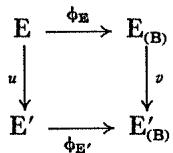
\includegraphics[keepaspectratio]{images/part002_74d11806.jpg}}

where \(\phi_{\mathbf{E}}\) and \(\phi_{\mathbf{E}'}\) are the canonical mappings.

It suffices to apply Proposition 1 to the A-homomorphism \(\phi_{\mathbf{E}'} \circ u: \mathbf{E} \to \mathbf{E}_{(\mathbf{B})}'\) .

The mapping \(v\) defined in the above corollary is denoted by \(\rho^{*}(u)\) or \(u_{(B)}\) . If \(E''\) is a third left A-module and \(v: E' \to E''\) an A-linear mapping, it is immediate that

\[
\left(v \circ u\right) _ {(\mathbf {B})} = v _ {(\mathbf {B})} \circ u _ {(\mathbf {B})}.
\]

Extending the ring of operators of a module is a transitive operation; to be precise:

PROPOSITION 2. Let \(\rho: \mathbf{A} \to \mathbf{B}\) , \(\sigma: \mathbf{B} \to \mathbf{C}\) be ring homomorphisms. For every left A-module E, there exists one and only one C-homomorphism

\[
\sigma^ {*} (\rho^ {*} (\mathrm{E})) \rightarrow (\sigma \circ \rho) ^ {*} (\mathrm{E})\tag{4}
\]

mapping \(1 \otimes (1 \otimes x)\) to \(1 \otimes x\) for all \(x \in E\) and this homomorphism is bijective.

The underlying Z-modules of \(\sigma^{*}(\rho^{*}(\mathbf{E}))\) and \((\sigma \circ \rho)^{*}(\mathbf{E})\) are respectively \(\mathbf{C} \otimes_{\mathbf{B}} (\mathbf{B} \otimes_{\mathbf{A}} \mathbf{E})\) and \(\mathbf{C} \otimes_{\mathbf{A}} \mathbf{E}\) . There exists a canonical Z-isomorphism \(\mathbf{C} \otimes_{\mathbf{B}} (\mathbf{B} \otimes_{\mathbf{A}} \mathbf{E}) \to (\mathbf{C} \otimes_{\mathbf{B}} \mathbf{B}) \otimes_{\mathbf{A}} \mathbf{E}\) (§ 3, no. 8, Proposition 8), which is also a C-isomorphism for the left C-module structures on both sides. Moreover, the C-module C ⊗B B is canonically identified with the C-module Cs under the isomorphism which maps γ ⊗ β to γσ(β) (§ 3, no. 4, Proposition 4) and this isomorphism is also an isomorphism for the right A-module structure on C ⊗B B defined by ρ and the right A-module structure on C defined by σ ∘ ρ. Thus a canonical isomorphism

\[
(\mathbf {C} \otimes_ {\mathbf {B}} \mathbf {B}) \otimes_ {\mathbf {A}} \mathbf {E} \rightarrow \mathbf {C} \otimes_ {\mathbf {A}} \mathbf {E}
\]

is obtained and, composing it with the isomorphism

\[
\mathbf {C} \otimes_ {\mathbf {B}} (\mathbf {B} \otimes_ {\mathbf {A}} \mathbf {E}) \rightarrow (\mathbf {C} \otimes_ {\mathbf {B}} \mathbf {B}) \otimes_ {\mathbf {A}} \mathbf {E}
\]

defined earlier, the desired canonical isomorphism is obtained.

If \(\phi, \phi'\) and \(\phi''\) denote the canonical mappings \(E \to \rho^*(E)\) , \(\rho^*(E \to) \sigma^*(\rho^*(E))\) and \(E \to (\sigma \circ \rho)^*(E)\) , \(\phi' \circ \phi\) is identified with \(\phi''\) under the canonical isomorphism of Proposition 2.

PROPOSITION 3. Let A, B be two commutative rings, \(\rho: \mathbf{A} \to \mathbf{B}\) a ring homomorphism and E, E' two A-modules. There exists one and only one B-homomorphism

\[
\mathbf {E} _ {(\mathbf {B})} \otimes_ {\mathbf {B}} \mathbf {E} _ {(\mathbf {B})} ^ {\prime} \rightarrow (\mathbf {E} \otimes_ {\mathbf {A}} \mathbf {E} ^ {\prime}) _ {(\mathbf {B})}\tag{5}
\]

mapping \((1 \otimes x) \otimes (1 \otimes x')\) to \(1 \otimes (x \otimes x')\) for \(x \in \mathbf{E}\) , \(x' \in \mathbf{E}'\) , and this homomorphism is bijective.

The left hand side of (5) may be written \((\mathbf{B} \otimes_{\mathbf{A}} \mathbf{E}) \otimes_{\mathbf{B}} (\mathbf{B} \otimes_{\mathbf{A}} \mathbf{E}')\) and is identified with \((\mathbf{E} \otimes_{\mathbf{A}} \mathbf{B}) \otimes_{\mathbf{B}} (\mathbf{B} \otimes_{\mathbf{A}} \mathbf{E}')\) since A and B are commutative; the latter product is identified successively with \(\mathbf{E} \otimes_{\mathbf{A}} (\mathbf{B} \otimes_{\mathbf{B}} \mathbf{B}) \otimes_{\mathbf{A}} \mathbf{E}'\) , \(\mathbf{E} \otimes_{\mathbf{A}} (\mathbf{B} \otimes_{\mathbf{A}} \mathbf{E}')\) , \(\mathbf{E} \otimes_{\mathbf{A}} (\mathbf{E}' \otimes_{\mathbf{A}} \mathbf{B})\) and finally \((\mathbf{E} \otimes_{\mathbf{A}} \mathbf{E}') \otimes_{\mathbf{A}} \mathbf{B}\) , using the associativity of the tensor product (§ 3, no. 8, Proposition 8), Proposition 4, § 3, no. 4, and the commutativity of A and B. The desired isomorphism is the composition of the successive canonical isomorphisms.

Clearly if S is a generating system of E, the image of S under the canonical mapping \(E \rightarrow E_{(B)}\) is a generating system of \(E_{(B)}\) ; in particular, if E is a finitely generated A-module, \(E_{(B)}\) is a finitely generated B-module.

PROPOSITION 4. Let E be an A-module admitting a basis \((a_{\lambda})_{\lambda \in L}\) ; if \(\phi : x \mapsto 1 \otimes x\) is the canonical mapping of E into \(\rho^{*}(\mathbf{E})\) , then \((\phi(a_{\lambda}))_{\lambda \in L}\) is a basis of \(\rho^{*}(\mathbf{E})\) . If \(\rho\) is injective, so is \(\phi\) .

The first assertion follows immediately from § 3, no. 7, Corollary 1 to Proposition 7. Also, for every family \((\xi_{\lambda})_{\lambda \in L}\) of elements of A of finite support, \(\phi\left(\sum_{\lambda \in L} \xi_{\lambda} a_{\lambda}\right) = \sum_{\lambda \in L} \rho(\xi_{\lambda}) \phi(a_{\lambda})\) and the relation \(\phi\left(\sum_{\lambda \in L} \xi_{\lambda} a_{\lambda}\right) = 0\) is therefore equivalent to \(\rho(\xi_{\lambda}) = 0\) for all \(\lambda \in L\) , whence the second assertion.

COROLLARY. For every projective A-module E, the B-module \(\rho^{*}(\mathbf{E})\) is projective. If further \(\rho\) is injective, the canonical mapping of E into \(\rho^{*}(\mathbf{E})\) is injective.

By hypothesis there exists a free A-module M containing E and in which E admits a supplement F. It follows immediately from §3, no. 7, Proposition 7 that \(\mathbf{M}_{(\mathbf{B})}\) is identified with the direct sum of \(\mathbf{E}_{(\mathbf{B})}\) and \(\mathbf{F}_{(\mathbf{B})}\) and if \(\phi\) and \(\psi\) are the canonical mappings \(\mathbf{E} \to \mathbf{E}_{(\mathbf{B})}\) and \(\mathbf{F} \to \mathbf{F}_{(\mathbf{B})}\) , the canonical mapping \(\mathbf{M} \to \mathbf{M}_{(\mathbf{B})}\) is just \(x + y \mapsto \phi(x) + \psi(y)\) . The corollary follows immediately from Proposition 4 applied to the A-module M.

When E is a right A-module, we write similarly \(\rho^{*}(\mathbf{E}) = \mathbf{E} \otimes_{\mathbf{A}} \rho_{*}(\mathbf{B}_{s})\) , B being considered this time as an (A, B)-bimodule and the right B-module structure on \(\rho^{*}(\mathbf{E})\) being such that \((x \otimes \beta)\beta' = x \otimes (\beta\beta')\) for \(\beta \in B, \beta' \in B\) and \(x \in E\) . We leave to the reader the task of stating for right modules the results corresponding to those of this no. and the following.

Remark (4). Consider the left A-module \(\rho_{*}(B_{s})\) defined by \(\rho\) and for every left A-module E, consider the Z-module

\[
\tilde {\rho} (\mathbf {E}) = \operatorname{Hom} _ {\mathbf {A}} \left(\rho_ {*} \left(\mathbf {B} _ {s}\right), \mathbf {E}\right).\tag{6}
\]

As \(\rho_{*}(\mathbf{B}_{s})\) has a right B-module structure, a left B-module structure is derived on \(\tilde{\rho}(\mathbf{E})\) ( \(\S 1\) , no. 14) such that, if \(u \in \tilde{\rho}(\mathbf{E})\) and \(b' \in \mathbf{B}\) , \(b'u\) is the homomorphism \(b \mapsto u(bb')\) of \(\rho_{*}(\mathbf{B}_{s})\) into \(\mathbf{E}\) . We further define an A-linear mapping, called canonical

\[
\eta : \rho_ {*} (\tilde {\rho} (\mathbf {E})) \rightarrow \mathbf {E}\tag{7}
\]

associating with every homomorphism \(u \in \tilde{\rho}(\mathbf{E})\) the element \(u(1)\) in \(\mathbf{E}\) . As \(\mathbf{B}\) can be considered as an (A, B)-bimodule by means of \(\rho\) , for every left B-module \(\mathbf{F}\) , there is a canonical \(\mathbf{Z}\) -module isomorphism

\[
\operatorname{Hom} _ {\mathbf {A}} \left(\rho_ {*} (\mathrm{B} _ {s}) \otimes_ {\mathrm{B}} \mathrm{F}, \mathrm{E}\right)\rightarrow \operatorname{Hom} _ {\mathbf {B}} (\mathrm{F}, \operatorname{Hom} _ {\mathbf {A}} \left(\rho_ {*} (\mathrm{B} _ {s}), \mathrm{E}\right))
\]

(§ 1, no. 1, Proposition 1). As the left A-module \(\rho^{*}(B_{s}) \otimes_{B} F\) is canonically identified with \(\rho_{*}(F)\) by virtue of § 3, no. 4, Proposition 4, we obtain a canonical Z-module isomorphism, the inverse of the above

\[
\operatorname{Hom} _ {\mathbf {B}} (\mathbf {F}, \tilde {\rho} (\mathbf {E})) \rightarrow \operatorname{Hom} _ {\mathbf {A}} (\rho_ {*} (\mathbf {F}), \mathbf {E})\tag{8}
\]

which associates with every B-linear mapping g of F into \(\tilde{\rho}(\mathbf{E})\) the composite mapping \(\eta \circ g\) , considered as an A-linear mapping of \(\rho_{*}(\mathbf{F})\) into E. In particular, under the hypotheses of Proposition 2, if F is replaced by \(\sigma_{*}(\mathbf{C}_{s})\) , we obtain a canonical C-isomorphism

\[
\tilde {\sigma} (\tilde {\rho} (\mathbf {E})) \rightarrow (\sigma \circ \rho) ^ {\sim} (\mathbf {E}).\tag{9}
\]

\subsection{RELATIONS BETWEEN RESTRICTION AND EXTENSION OF THE RING OF SCALARS}

Let \(\rho: \mathbf{A} \to \mathbf{B}\) be a ring homomorphism. For every left A-module E, a canonical A-linear mapping

\[
\phi_ {\mathbf {E}}: \mathbf {E} \rightarrow \rho_ {*} (\rho^ {*} (\mathbf {E}))\tag{10}
\]

was defined in no. 1 such that \(\phi_{\mathbb{E}}(x) = 1 \otimes x\) . We consider now a left B-module F and apply Proposition 1 (no. 1) to the A homomorphism \(\mathbf{l}_{\rho_{*}(\mathbf{F})}: \rho_{*}(\mathbf{F}) \to \rho_{*}(\mathbf{F})\) : we obtain a B-linear mapping

\[
\psi_ {\mathbf {F}} \colon \rho^ {*} (\rho_ {*} (\mathbf {F})) \rightarrow \mathbf {F}\tag{11}
\]

equal to \(\delta(1_{\rho_*(\mathbb{F})})\) and such therefore that, for all \(y \in \mathbb{F}\) and all \(\beta \in \mathbb{B}\) , \(\psi_{\mathbb{F}}(\beta \otimes y) = \beta y\) .

PROPOSITION 5. Let E be a left A-module and F a left B-module; the composite mappings

\[
\rho^ {*} (\mathrm{E}) \xrightarrow [ \rho^ {*} (\phi_ {\mathrm{E}}) ]{} \rho^ {*} (\rho_ {*} (\rho^ {*} (\mathrm{E}))) \xrightarrow [ \psi_ {\rho^ {*} (\mathrm{E})} ]{} \rho^ {*} (\mathrm{E})\tag{12}
\]

\[
\rho_ {*} (\mathrm{F}) \xrightarrow [ \phi_ {\rho_ {*} (\mathrm{F})} ]{} \rho_ {*} (\rho^ {*} (\rho_ {*} (\mathrm{F}))) \xrightarrow [ \rho_ {*} (\psi_ {\mathrm{F}}) ]{} \rho_ {*} (\mathrm{F})\tag{13}
\]

are respectively equal to the identity mappings of \(\rho^{*}(\mathbf{E})\) and \(\rho_{*}(\mathbf{F})\) .

We give the proof, for example, for (12); for all \(x \in \mathbf{E}\) , the mapping \(\rho^{*}(\phi_{\mathbf{E}})\) maps \(1 \otimes x\) to the element \(1 \otimes (1 \otimes x)\) and the mapping \(\psi_{\rho^{*}(\mathbf{E})}\) maps \(1 \otimes (1 \otimes x)\) to the element \(1 \otimes x\) ; the conclusion follows from the fact that the elements of the form \(1 \otimes x\) generate the B-module \(\rho^{*}(\mathbf{E})\) ; the proof is even simpler for (13).

COROLLARY. The mappings \(\rho^{*}(\phi_{\mathbf{E}})\) and \(\phi_{\rho^{*}(\mathbf{F})}\) are injective and respectively identify \(\rho^{*}(\mathbf{E})\) with a direct factor of \(\rho^{*}(\rho_{*}(\rho^{*}(\mathbf{E})))\) and \(\rho_{*}(\mathbf{F})\) with a direct factor of \(\rho_{*}(\rho^{*}(\rho_{*}(\mathbf{F})))\) .

This is a consequence of Proposition 5 and §1, no. 9, Corollary 2 to Proposition 15.

PROPOSITION 6. Let E be a left A-module and F a right B-module. There exists one and only one Z-homomorphism

\[
\rho_ {*} (\mathrm{F}) \otimes_ {\mathrm{A}} \mathrm{E} \rightarrow \mathrm{F} \otimes_ {\mathrm{B}} \rho^ {*} (\mathrm{E})\tag{14}
\]

mapping \(y \otimes x\) to \(y \otimes (1 \otimes x)\) for all \(x \in E\) and all \(y \in F\) and this homomorphism is bijective.

By definition the right hand side of (14) is \(F \otimes_{B} (B \otimes_{A} E)\) , where B is considered as a (B, A)-bimodule, and there is a canonical Z-isomorphism \((\mathbf{F} \otimes_{\mathbf{B}} \mathbf{B}) \otimes_{\mathbf{A}} \mathbf{E} \to \mathbf{F} \otimes_{\mathbf{B}} (\mathbf{B} \otimes_{\mathbf{A}} \mathbf{E})\) defined in §3, no. 8, Proposition 8; on the other hand, the canonical isomorphism \(F \to F \otimes_{B} B\) of §3, no. 4, Proposition 4 is an isomorphism for the right A-module structures on the two sides, defined by \(\rho\) . Whence the desired isomorphism.

When A and B are commutative, the isomorphism (14) is an A-module isomorphism

\[
\rho_ {*} (\mathrm{F}) \otimes_ {\mathrm{A}} \mathrm{E} \rightarrow \rho_ {*} (\mathrm{F} \otimes_ {\mathrm{B}} \rho^ {*} (\mathrm{E})).
\]

\subsection{EXTENSION OF THE RING OF OPERATORS OF A HOMOMORPHISM MODULE}

Let A be a commutative ring, B a ring, \(\rho: \mathbf{A} \to \mathbf{B}\) a ring homomorphism and E, F two A-modules; as B is an (A, A)-bimodule (by means of \(\rho\) ) and F can be considered as an (A, A)-bimodule, there are on the Z-module B \(\otimes_{\mathbf{A}}\) F two A-module structures, under which respectively \(a(b \otimes y) = (\rho(a)b) \otimes y\) and \(a(b \otimes y) = b \otimes (ay)\) for \(a \in \mathbf{A}\) , \(b \in \mathbf{B}\) , \(y \in \mathbf{F}\) . We shall denote the two A-modules thus defined by G' and G''; G' is moreover just the A-module \(\rho_*(\rho^*(\mathbf{F}))\) .

This being so, in the definition of the canonical homomorphism of § 4, no. 2, formula (7), we replace B by A, the B-module F by the ring B considered as an A-module by means of \(\rho\) and G by F considered as an (A, A)-bimodule; as A is commutative, we may write the canonical Z-homomorphism obtained as

\[
\mathbf {B} \otimes_ {\mathbf {A}} \operatorname{Hom} _ {\mathbf {A}} (\mathbf {E}, \mathbf {F}) \rightarrow \operatorname{Hom} _ {\mathbf {A}} (\mathbf {E}, \mathbf {G} ^ {\prime \prime}).\tag{15}
\]

On the other hand (no. 1, formula (2)), there is a canonical Z-isomorphism

\[
\mathrm{Hom} _ {\mathbf {A}} (\mathbf {E}, \mathbf {G} ^ {\prime}) = \mathrm{Hom} _ {\mathbf {A}} (\mathbf {E}, \rho_ {*} (\rho^ {*} (\mathbf {F}))) \rightarrow \mathrm{Hom} _ {\mathbf {B}} (\rho^ {*} (\mathbf {E}), \rho^ {*} (\mathbf {F})). \tag {16}
\]

Suppose now that \(\rho(A)\) is contained in the centre of \(B\) , in which case \(\rho\) is also called a central homomorphism \(*\) (or \(\rho\) is said to define an A-algebra structure on \(B\) , cf.~III, §1, no. 3). Then the A-module structures of \(G'\) and \(G''\) are identical and composing the homomorphisms (16) and (15) we thus obtain a canonical Z-homomorphism

\[
\omega : \mathrm{B} \otimes_ {\mathrm{A}} \operatorname{Hom} _ {\mathrm{A}} (\mathrm{E}, \mathrm{F}) \rightarrow \operatorname{Hom} _ {\mathrm{B}} \left(\mathrm{E} _ {(\mathrm{B})}, \mathrm{F} _ {(\mathrm{B})}\right)\tag{17}
\]

which is characterized by the fact that, for all \(u \in \operatorname{Hom}_{\mathbf{A}}(\mathbf{E}, \mathbf{F})\) and all \(b \in B\)

\[
\omega (b \otimes u) = r _ {b} \otimes u,\tag{18}
\]

where \(r_b\) denotes right multiplication by \(b\) in B.

Moreover, the hypothesis that \(\omega\) is a central homomorphism implies that \((bb')\rho(a) = b\rho(a)b'\) for \(b, b'\) in B and \(a \in A\) ; in other words the right B-module structure of \(B_d\) is compatible with its A-module structure; it thus defines on B \(\otimes_A\) \(\mathrm{Hom}_{\mathbf{A}}(\mathbf{E}, \mathbf{F})\) a right B-module structure (§ 3, no. 4) and also on \(\mathrm{F}_{(\mathbf{B})} = \mathbf{B} \otimes_{\mathbf{A}} \mathbf{F}\) , and finally, as the left and right B-module structures on \(\mathrm{F}_{(\mathbf{B})}\) are compatible, a right B-module structure is also obtained on \(\mathrm{Hom}_{\mathbf{B}}(\mathrm{E}_{(\mathbf{B})}, \mathrm{F}_{(\mathbf{B})})\) (§ 1, no. 14). Then it is immediately verified that (17) is a right B-module homomorphism for these structures.

PROPOSITION 7. Let A be a commutative ring, B a ring, \(\rho: \mathbf{A} \to \mathbf{B}\) a central homomorphism and E, F two A-modules.

\begin{enumerate}
\def\labelenumi{(\roman{enumi})}
\item
  If B is a projective (resp. finitely generated projective) A-module, the homomorphism (17) is injective (resp. bijective).
\item
  If \(\mathbf{E}\) is a finitely generated projective A-module, the homomorphism (17) is bijective.
\end{enumerate}

As (16) is bijective, the proposition follows from § 4, no. 2. Proposition 2, applied to the canonical homomorphism (15).

\subsection{DUAL OF A MODULE OBTAINED BY EXTENSION OF SCALARS}

Let A, B be two rings, \(\rho: \mathbf{A} \to \mathbf{B}\) a ring homomorphism, E a left A-module and \(\mathbf{E}^*\) its dual. We shall define a canonical B-linear mapping

\[
\nu _ {E}: (E ^ {*}) _ {(B)} \rightarrow (E _ {(B)}) ^ {*}.\tag{19}
\]

The left hand side of (19) may be written as \(\mathrm{Hom}_{\mathbf{A}}(\mathbf{E},\mathbf{A})\otimes_{\mathbf{A}}\rho_{*}(\mathbf{B}_{s})\) , where, in \(\mathrm{Hom}_{\mathbf{A}}(\mathbf{E},\mathbf{A})\) , \(\mathbf{A}\) is considered as an \((\mathbf{A},\mathbf{A})\) -bimodule. Then there is a canonical \(\mathbf{Z}\) -homomorphism ( \(\S 4\) , no. 2, formula (7))

\[
\nu: \operatorname{Hom} _ {A} (E, A) \otimes_ {A} \rho_ {*} (B _ {s}) \rightarrow \operatorname{Hom} _ {A} (E, A \otimes_ {A} \rho_ {*} (B _ {s})) = \operatorname{Hom} _ {A} (E, \rho_ {*} (B _ {s}))
\]

with the identification given by the canonical isomorphism of § 3, no. 4, Proposition 4. On the other hand, the right hand side of (19) may be written as \(\mathrm{Hom}_{\mathbf{B}}(\rho_{*}(\mathbf{B}_{d}) \otimes_{\mathbf{A}} \mathbf{E}, \mathbf{B}_{s})\) ; as B is a (B, A)-bimodule, there is a canonical Z-isomorphism (§ 4, no. 1, Proposition 1)

\[
\beta : \operatorname{Hom} _ {\mathbf {B}} (\rho_ {*} (\mathbf {B} _ {d}) \otimes_ {\mathbf {A}} \mathbf {E}, \mathbf {B} _ {s}) \rightarrow \operatorname{Hom} _ {\mathbf {A}} (\mathbf {E}, \operatorname{Hom} _ {\mathbf {B}} (\mathbf {B} _ {s}, \mathbf {B} _ {s}))
\]

and \(\mathrm{Hom}_{\mathbb{B}}(\mathbf{B}_s,\mathbf{B}_s)\) is canonically identified, as an A-module, with \(\rho_{*}(\mathbf{B}_{s})\) (see the proof of no. 1, Proposition 1). Taking account of these identifications, we obtain the homomorphism \(\nu_{\mathbb{E}}\) ; it is easily verified that this homomorphism is characterized by the equation

\[
\langle \xi \otimes x, \nu _ {E} (x ^ {*} \otimes \eta) \rangle = \xi_ {\rho} (\langle x, x ^ {*} \rangle) \eta ,\tag{20}
\]

for \(x \in \mathbf{E}\) , \(x^{*} \in \mathbf{E}^{*}\) , \(\xi\) , \(\eta\) in \(\mathbf{B}\) , which shows immediately that \(\nu_{\mathbf{E}}\) is B-linear. Moreover, for every A-linear mapping \(u: \mathbf{E} \to \mathbf{F}\) the diagram

\[
\begin{array}{c c c} (\mathrm{F} ^ {*}) _ {(\mathrm{B})} & \xrightarrow {\nu_ {\mathrm{F}}} & (\mathrm{F} _ {(\mathrm{B})}) ^ {*} \\ \Big \downarrow^ {(t _ {u}) _ {(\mathrm{B})}} & & \Big \downarrow^ {t (u _ {(\mathrm{B})})} \\ (\mathrm{E} ^ {*}) _ {(\mathrm{B})} & \xrightarrow {\nu_ {\mathrm{E}}} & (\mathrm{E} _ {(\mathrm{B})}) ^ {*} \end{array}
\]

is commutative.

PROPOSITION 8. If one of the A-modules E, \(\rho_{*}(B_{s})\) is projective and finitely generated, the homomorphism \(\nu_{\mathbb{E}}\) is bijective.

This follows from the above and § 4, no. 2, Proposition 2.

Suppose in particular that E is a finitely generated free A-module and let \((e_{i})_{1\leqslant i\leqslant n}\) be a basis of E and \((e_{i}^{*})\) the dual basis; then the canonical isomorphism (19) maps the basis \((e_{i}^{*}\otimes1)\) of \((\mathrm{E}^{*})_{(\mathrm{B})}\) to the dual basis of the basis \((1\otimes e_{i})\) of \(\mathrm{E}_{(\mathrm{B})}\) .

\subsection{A CRITERION FOR FINITENESS}

PROPOSITION 9. Let B be a ring, A a subring of B and P a projective left A-module. Then, if \(P_{(B)}\) is a finitely generated B-module, P is itself a finitely generated A-module.

We know (§ 2, no. 6, Proposition 12) that there exists a family \((a_{\lambda})_{\lambda \in L}\) of elements of P and a family \((a_{\lambda}^{*})_{\lambda \in L}\) of elements of the dual P* such that, for all \(x \in \mathbb{P}\) , the family \((\langle x, a_{\lambda}^{*} \rangle)\) is of finite support and \(x = \sum_{\lambda} \langle x, a_{\lambda}^{*} \rangle a_{\lambda}\) . Since \(\mathrm{P}_{(\mathbb{B})}\) is finitely generated, there exists a finite family \((y_{i})_{i \in I}\) of elements of P such that \(\mathrm{P}_{(\mathbb{B})}\) is generated by the elements \(1 \otimes y_{i}\) . For each index \(i\) , the family \((\langle y_{i}, a_{\lambda}^{*} \rangle)\) has finite support. Hence there exists a finite subset H of L such that \(\langle y_{i}, a_{\lambda}^{*} \rangle = 0\) for \(i \in I\) and \(\lambda \notin H\) . Since

\[
\langle 1 \otimes y _ {i}, 1 d _ {\mathrm{B}} \otimes a _ {\lambda} ^ {*} \rangle = \langle y _ {i}, a _ {\lambda} ^ {*} \rangle ,
\]

it follows that \(1d_{\mathbf{B}} \otimes a_{\lambda}^{*} = 0\) for \(\lambda \notin \mathbf{H}\) . Hence, for all \(x \in \mathbf{P}\) ,

\[
\langle x, a _ {\lambda} ^ {*} \rangle = \langle 1 \otimes x, 1 _ {B} \otimes a _ {\lambda} ^ {*} \rangle = 0
\]

for \(\lambda \notin \mathbf{H}\) . This shows that the A-module \(\mathbf{P}\) is generated by the \(a_{\lambda}\) such that \(\lambda \in \mathbf{H}\) .

\section{INVERSE AND DIRECT LIMITS OF MODULES}

Throughout this paragraph, I will denote a non-empty preordered set and \(\alpha \leqslant \beta\) the preorder relation on I. Unless otherwise mentioned, the inverse and direct systems have indexing set I.

\subsection{INVERSE LIMITS OF MODULES}

Let \((\mathbf{A}_{\alpha}, \phi_{\alpha\beta})\) be an inverse system of rings (I, § 10, no. 1), \((\mathbf{E}_{\alpha}, f_{\alpha\beta})\) an inverse system of commutative groups (written additively) (I, § 10, no. 1) and suppose that each \(E_{\alpha}\) has a left \(A_{\alpha}\) -module structure; moreover suppose that for \(\alpha \leqslant \beta\) \((f_{\alpha\beta}, \phi_{\alpha\beta})\) is a dimorphism of \(E_{\beta}\) into \(E_{\alpha}\) (§ 1, no. 13), in other words that

\[
f _ {\alpha \beta} (\lambda_ {\beta} x _ {\beta}) = \phi_ {\alpha \beta} (\lambda_ {\beta}) f _ {\alpha \beta} (x _ {\beta}),\tag{1}
\]

for \(x_{\beta} \in \mathrm{E}_{\beta}, \lambda_{\beta} \in \mathrm{A}_{\beta}\) ; then it follows from I, § 10, no. 2 that \(\mathbf{E} = \varprojlim \mathbf{E}_{\alpha}\) has a left module structure over \(\mathbf{A} = \varprojlim \mathbf{A}_{\alpha}\) . For all \(\alpha \in \mathbf{I}\) , let \(f: \mathbf{E} \to \mathbf{E}_{\alpha}, \phi_{\alpha}: \mathbf{A} \to \mathbf{A}_{\alpha}\) be the canonical mappings; then \((f_{\alpha}, \phi_{\alpha})\) is a dimorphism of \(\mathbf{E}\) into \(\mathbf{E}_{\alpha}\) . We shall say that \((\mathbf{E}_{\alpha}, f_{\alpha\beta})\) is an inverse system of left \(A_{\alpha}\) -modules and that the A-module E is its inverse limit.

Let \((\mathbf{E}_{\alpha}^{\prime}, f_{\alpha\beta}^{\prime})\) be another inverse system of left \(A_{\alpha}\) -modules and, for all \(\alpha\) , let \(u_{\alpha}: E_{\alpha}^{\prime} \to E_{\alpha}\) be an \(A_{\alpha}\) -linear mapping, these mappings forming an inverse system; then \(u = \lim_{\leftarrow} u_{\alpha}\) is an A-linear mapping of \(\lim_{\leftarrow} E_{\alpha}^{\prime}\) into \(\lim_{\leftarrow} E_{\alpha}\) .

Moreover:

PROPOSITION 1. Let \((\mathbf{E}_{\alpha}, f_{\alpha\beta})\) , \((\mathbf{E}_{\alpha}^{\prime}, f_{\alpha\beta}^{\prime})\) , \((\mathbf{E}_{\alpha}^{\prime \prime}, f_{\alpha\beta}^{\prime \prime})\) be three inverse systems of \(\mathbf{A}_{\alpha}\) -modules and \((u_{\alpha})\) , \((v_{\alpha})\) two inverse systems of \(\mathbf{A}_{\alpha}\) -linear mappings such that the sequences

\[
0 \longrightarrow \mathrm{E} _ {\alpha} ^ {\prime} \stackrel {u _ {\alpha}} {\longrightarrow} \mathrm{E} _ {\alpha} \stackrel {v _ {\alpha}} {\longrightarrow} \mathrm{E} _ {\alpha} ^ {\prime \prime}
\]

are exact for all \(\alpha\) . Then, writing \(u = \varprojlim u_{\alpha}\) , \(v = \varprojlim v_{\alpha}\) , the sequence

\[
0 \longrightarrow \varprojlim \mathrm{E} _ {\alpha} ^ {\prime} \stackrel {u} {\longrightarrow} \varprojlim \mathrm{E} _ {\alpha} \stackrel {v} {\longrightarrow} \varprojlim \mathrm{E} _ {\alpha} ^ {\prime \prime}
\]

is exact.

As \(u_{\alpha}^{-1}(0) = \{0\}\) for all \(\alpha\) , it follows from Set Theory, III, § 7, no. 2, Proposition 2 that \(u^{-1}(0) = \{0\}\) , hence \(u\) is injective; further, the \(u_{\alpha}(\mathrm{E}_{\alpha}')\) form an inverse system of subsets of the \(\mathrm{E}_{\alpha}\) and thus \(u(\varprojlim \mathrm{E}_{\alpha}') = \varprojlim u_{\alpha}(\mathrm{E}_{\alpha}')\) . As \(u_{\alpha}(\mathrm{E}_{\alpha}') = v_{\alpha}^{-1}(0)\) by hypothesis, \(v^{-1}(0) = \varprojlim u_{\alpha}(\mathrm{E}_{\alpha}') = u(\varprojlim \mathrm{E}_{\alpha}')\) (Set Theory, III, § 7, no. 2, Proposition 2), which completes the proof.

Remarks. (1) Proposition 1 and its proof are valid for arbitrary groups, except for change of notation.

\begin{enumerate}
\def\labelenumi{(\arabic{enumi})}
\setcounter{enumi}{1}
\tightlist
\item
  Note that if there are exact sequences
\end{enumerate}

\[
0 \longrightarrow \mathrm{E} _ {\alpha} ^ {\prime} \stackrel {u _ {\alpha}} {\longrightarrow} \mathrm{E} _ {\alpha} \stackrel {v _ {\alpha}} {\longrightarrow} \mathrm{E} _ {\alpha} ^ {\prime \prime} \longrightarrow 0
\]

it does not necessarily follow that the sequence

\[
0 \longrightarrow \varprojlim \mathrm{E} _ {\alpha} ^ {\prime} \stackrel {u} {\longrightarrow} \varprojlim \mathrm{E} _ {\alpha} \stackrel {v} {\longrightarrow} \varprojlim \mathrm{E} _ {\alpha} ^ {\prime \prime} \longrightarrow 0
\]

is exact; in other words, the inverse limit of an inverse system of surjective linear mappings is not necessarily surjective (cf.~Exercise 1).

Suppose now that the \(\mathbf{A}_{\alpha}\) are equal to the same ring \(\mathbf{A}\) and the \(\phi_{\alpha \beta}\) to \(1_{\mathbf{A}}\) ; then for every inverse system \((\mathrm{E}_{\alpha}, f_{\alpha \beta})\) of A-modules, \(\mathbf{E} = \varprojlim \mathbf{E}_{\alpha}\) is an A-module. Let \(\mathbf{F}\) be an A-module and, for all \(\alpha\) , let \(u_{\alpha}: \mathbf{F} \to \mathbf{E}_{\alpha}\) be an A-linear mapping such that \((u_{\alpha})\) is an inverse system of mappings; then \(u = \varprojlim u_{\alpha}\) is an A-linear mapping of \(\mathbf{F}\) into \(\varprojlim \mathbf{E}_{\alpha}\) . Conversely, for every A-linear mapping \(v: \mathbf{F} \to \varprojlim \mathbf{E}_{\alpha}\) , the family of \(v_{\alpha} = f_{\alpha} \circ v\) is an inverse system of A-linear mappings such that \(v = \varprojlim v_{\alpha}\) . We note on the other hand that for \(\alpha \leqslant \beta\) the mapping

\[
\operatorname{Hom} \left(\mathrm{l} _ {\mathrm{F}}, f _ {\alpha \beta}\right) = \bar {f} _ {\alpha \beta}: \operatorname{Hom} _ {\mathrm{A}} (\mathrm{F}, \mathrm{E} _ {\beta}) \rightarrow \operatorname{Hom} _ {\mathrm{A}} (\mathrm{F}, \mathrm{E} _ {\alpha})
\]

is a Z-module homomorphism such that \((\mathrm{Hom}_{\mathbf{A}}(\mathrm{F}, \mathrm{E}_{\alpha}), \vec{f}_{\alpha\beta})\) is an inverse system of Z-modules; as \(\vec{f}_{\alpha\beta}(v_{\beta}) = f_{\alpha\beta} \circ v_{\beta}\) , the above remarks can therefore be expressed as follows:

PROPOSITION 2. For every inverse system \((\mathbf{E}_{\alpha}, f_{\alpha \beta})\) of A-modules and every A-module F, the canonical mapping \(u \mapsto (f_{\alpha} \circ u)\) is a Z-module isomorphism

\[
l _ {\mathrm{F}}: \operatorname{Hom} _ {\mathrm{A}} (\mathrm{F}, \varprojlim \mathrm{E} _ {\alpha}) \rightarrow \varprojlim \operatorname{Hom} _ {\mathrm{A}} (\mathrm{F}, \mathrm{E} _ {\alpha}).\tag{2}
\]

COROLLARY. For every A-module homomorphism \(v: \mathbf{F} \to \mathbf{F}'\) , the

\[
\bar {v} _ {\alpha} = \operatorname{Hom} (v, 1 _ {\mathrm{E} _ {\alpha}}): \operatorname{Hom} (\mathrm{F} ^ {\prime}, \mathrm{E} _ {\alpha}) \rightarrow \operatorname{Hom} (\mathrm{F}, \mathrm{E} _ {\alpha})
\]

form an inverse system of Z-linear mappings and the diagram

\[
\begin{array}{c} \operatorname{Hom} (\mathrm{F} ^ {\prime}, \varprojlim \mathrm{E} _ {\alpha}) \xrightarrow {l _ {\mathrm{F} ^ {\prime}}} \varprojlim \operatorname{Hom} (\mathrm{F} ^ {\prime}, \mathrm{E} _ {\alpha}) \\ \operatorname{Hom} (v, 1 _ {\mathrm{E}}) \Biggl \downarrow \qquad \qquad \qquad \qquad \qquad \qquad \qquad \qquad \qquad \qquad \qquad \qquad \qquad \qquad \qquad \qquad \qquad \qquad \qquad \qquad \qquad \qquad \qquad \qquad \qquad \qquad \qquad \qquad \qquad \qquad \qquad \qquad \qquad \qquad \\ \operatorname{Hom} (\mathrm{F}, \varprojlim \mathrm{E} _ {\alpha}) \xrightarrow {l _ {\mathrm{F}}} \varprojlim \operatorname{Hom} (\mathrm{F}, \mathrm{E} _ {\alpha}) \end{array}\tag{3}
\]

is commutative.

For all \(u \in \operatorname{Hom}(\mathbf{F}', \varprojlim \mathbf{E}_{\alpha})\) , \(l_{\mathbf{F}}(u \circ v) = (f_{\alpha} \circ u \circ v)\) by definition and the commutativity of diagram (3) follows immediately from the definitions.

\subsection{DIRECT LIMITS OF MODULES}

\BourbakiRunInHeading{Henceforth I is assumed to be right directed.}

Let \((\mathbf{A}_{\alpha}, \phi_{\beta\alpha})\) be a direct system of rings (I, § 10, no. 3), \((\mathbf{E}_{\alpha}, f_{\beta\alpha})\) a direct system of commutative groups (written additively) (I, § 10, no. 3) and suppose that each \(E_{\alpha}\) has a left \(A_{\alpha}\) -module structure; further, suppose that, for \(\alpha \leqslant \beta\) , \((f_{\beta\alpha}, \phi_{\beta\alpha})\) is a dimorphism of \(E_{\alpha}\) into \(E_{\beta}\) (§ 1, no. 13), in other words that

\[
f _ {\beta \alpha} (\lambda_ {\alpha} x _ {\alpha}) = \phi_ {\beta \alpha} (\lambda_ {\alpha}) f _ {\beta \alpha} (x _ {\alpha})\tag{4}
\]

for \(x_{\alpha} \in \mathrm{E}_{\alpha}, \lambda_{\alpha} \in \mathrm{A}_{\alpha}\) ; then \(\mathbf{E} = \varinjlim \mathbf{E}_{\alpha}\) has a left module structure over \(\mathbf{A} = \varinjlim \mathbf{A}_{\alpha}\) (I, § 10, no. 4). For all \(\alpha \in \mathbf{I}\) , let \(f_{\alpha}: \mathrm{E}_{\alpha} \to \mathrm{E}\) , \(\phi_{\alpha}: \mathrm{A}_{\alpha} \to \mathrm{A}\) be the canonical mappings; then \((f_{\alpha}, \phi_{\alpha})\) is a dimorphism of \(\mathbf{E}_{\alpha}\) into \(\mathbf{E}\) . We shall say that \((\mathbf{E}_{\alpha}, f_{\beta \alpha})\) is a direct system of left \(\mathbf{A}_{\alpha}\) -modules and that the A-module \(\mathbf{E}\) is its direct limit.

Let \((\mathbf{E}_{\alpha}^{\prime}, f_{\beta \alpha}^{\prime})\) be another direct system of left \(A_{\alpha}\) -modules and, for all \(\alpha\) , let \(u_{\alpha}: \mathrm{E}_{\alpha}' \to \mathrm{E}_{\alpha}\) be an \(\mathbf{A}_{\alpha}\) -linear mapping, these mappings forming a direct system; then \(u = \varinjlim u_{\alpha}\) is an A-linear mapping of \(\varinjlim \mathrm{E}_{\alpha}'\) into \(\varinjlim \mathrm{E}_{\alpha}\) .

Moreover:

PROPOSITION 3. Let \((\mathbf{E}_{\alpha}, f_{\beta \alpha})\) , \((\mathbf{E}_{\alpha}', f_{\beta \alpha}')\) , \((\mathbf{E}_{\alpha}'', f_{\beta \alpha}'')\) be three direct systems of \(\mathbf{A}_{\alpha}\) -modules and \((u_{\alpha})\) , \((v_{\alpha})\) two direct systems of \(\mathbf{A}_{\alpha}\) -linear mappings such that the sequences

\[
\mathrm{E} _ {\alpha} ^ {\prime} \xrightarrow {u _ {\alpha}} \mathrm{E} _ {\alpha} \xrightarrow {v _ {\alpha}} \mathrm{E} _ {\alpha} ^ {\prime \prime}
\]

are exact for all \(\alpha\) . Then, writing \(u = \varinjlim u_{\alpha}\) , \(v = \varinjlim v_{\alpha}\) , the sequence

\[
\lim _ {\longrightarrow} \mathrm{E} _ {\alpha} ^ {\prime} \xrightarrow {u} \lim _ {\longrightarrow} \mathrm{E} _ {\alpha} \xrightarrow {v} \lim _ {\longrightarrow} \mathrm{E} _ {\alpha} ^ {\prime \prime}
\]

is exact.

\(u(\varinjlim \mathrm{E}_{\alpha}^{\prime}) = \varinjlim u_{\alpha}(\mathrm{E}_{\alpha}^{\prime})\) and \(v^{-1}(0) = \varinjlim v_{\alpha}^{-1}(0)\) (Set Theory, III, § 7, no. 6, Corollary to Proposition 7).

Loosely speaking, Proposition 3 can also be expressed by saying that passing to the direct limit preserves exactness.

PROPOSITION 4. Let \((\mathbf{E}_{\alpha}, f_{\beta \alpha})\) be a direct system of \(\mathbf{A}_{\alpha}\) -modules, \(\mathbf{E} = \varinjlim \mathbf{E}_{\alpha}\) its direct limit and \(\phi_{\alpha}: \mathbf{A}_{\alpha} \to \mathbf{A}\) and \(f_{\alpha}: \mathbf{E}_{\alpha} \to \mathbf{E}\) the canonical mappings for all \(\alpha \in \mathbf{I}\) . If, for all \(\alpha \in \mathbf{I}\) , \(\mathbf{S}_{\alpha}\) is a generating system of \(\mathbf{E}_{\alpha}\) , then \(\mathbf{S} = \bigcup_{\alpha \in \mathbf{I}} f_{\alpha}(\mathbf{S}_{\alpha})\) is a generating system of \(\mathbf{E}\) .

Every \(x \in \mathbf{E}\) is of the form \(f_{\alpha}(x_{\alpha})\) for some \(\alpha \in \mathbf{I}\) and some \(x_{\alpha} \in \mathbf{E}_{\alpha}\) and by hypothesis \(x = \sum_{i} \lambda_{\alpha}^{(i)} y_{\alpha}^{(i)}\) , where \(\lambda_{\alpha}^{(i)} \in \mathbf{A}_{\alpha}\) and \(y_{\alpha}^{(i)} \in \mathbf{S}_{\alpha}\) ; writing \(\lambda^{(i)} = \phi_{\alpha}(\lambda_{\alpha}^{(i)})\) , \(y^{(i)} = f_{\alpha}(y_{\alpha}^{(i)})\) , we obtain \(x = \sum_{i} \lambda^{(i)} y^{(i)}\) .

PROPOSITION 5. With the hypotheses and notation of Proposition 4, suppose that for all \(\alpha \in I\) , \(E_{\alpha}\) is the direct sum of a family \((M_{\alpha}^{\lambda})_{\alpha \in L}\) of submodules (the indexing set \(L\) being independent of \(\alpha\) ) and that \(f_{\beta \alpha}(M_{\alpha}^{\lambda}) \subset M_{\alpha}^{\lambda}\) for \(\alpha \leqslant \beta\) and for all \(\lambda \in L\) . Then \(E\) is the direct sum of the submodules \(M^{\lambda} = \varinjlim_{\alpha} M_{\alpha}^{\lambda} (\lambda \in L)\) .

It follows from Proposition 4 that E is the sum of the \(\mathbf{M}^{\lambda}\) . Let \((y^{\lambda})_{\lambda \in L}\) be a family such that \(y^{\lambda} \in \mathbf{M}^{\lambda}\) for all \(\lambda \in L\) and whose support is finite and suppose that \(\sum_{\lambda} y^{\lambda} = 0\) . By virtue of Set Theory, III, §7, no. 5, Lemma 1, there exist an \(\alpha \in I\) and a family \((x_{\alpha}^{\lambda})_{\alpha \in L}\) of finite support consisting of elements of \(\mathbf{E}_{\alpha}\) such that \(x_{\alpha}^{\lambda} \in \mathbf{M}_{\alpha}^{\lambda}\) and \(y^{\lambda} = f_{\alpha}(x_{\alpha}^{\lambda})\) for all \(\lambda \in L\) . The relation \(f_{\alpha}\left(\sum_{\lambda \in L} x_{\alpha}^{\lambda}\right) = 0\) implies the existence of a \(\beta \geqslant \alpha\) such that \(f_{\beta \alpha}\left(\sum_{\lambda \in L} x_{\alpha}^{\lambda}\right) = 0\) (Set Theory, III, § 7, no. 5, Lemma 1), which may be written as \(\sum_{\lambda \in L} x_{\beta}^{\lambda} = 0\) , where \(x_{\beta}^{\lambda} = f_{\beta \alpha}(x_{\alpha}^{\lambda}) \in \mathrm{M}_{\beta}^{\lambda}\) by hypothesis; hence \(x_{\beta}^{\lambda} = 0\) for all \(\lambda \in \mathbf{L}\) and therefore \(y^{\lambda} = f_{\beta}(x_{\beta}^{\lambda}) = 0\) for all \(\lambda \in \mathbf{L}\) , which proves that the sum of the \(\mathbf{M}^{\lambda}\) is direct.

COROLLARY. Let \((\mathbf{P}_{\alpha})\) be a direct system of subsets of \(\mathbf{E}_{\alpha}\) and let \(\mathbf{P} = \varinjlim \mathbf{P}_{\alpha}\) . If, for all \(\alpha \in \mathbf{I}\) , \(\mathbf{P}_{\alpha}\) is a free subset (resp. basis) of \(\mathbf{E}_{\alpha}\) , then \(\mathbf{P}\) is a free subset (resp. basis) of \(\mathbf{E}\) .

The second assertion follows immediately from the first and Proposition 4. It is therefore sufficient to prove that if the \(\mathbf{P}_{\alpha}\) are free every subset \(\{y^{(i)}\}_{1\leqslant i\leqslant n}\) consisting of distinct elements of \(\mathbf{P}\) , is free. There exists an \(\alpha \in \mathbf{I}\) and elements \(x_{\alpha}^{(i)}\in \mathbf{P}_{\alpha}\) such that \(y^{(i)} = f_{\alpha}(x_{\alpha}^{(i)})\) for \(1\leqslant i\leqslant n\) (Set Theory, III, §7, no. 5, Lemma 1); if \(\sum_{i}\lambda^{(i)}y^{(i)} = 0\) , it may be assumed that \(\lambda^{(i)} = \phi_{\alpha}(\lambda_{\alpha}^{(i)})\) for \(1\leqslant i\leqslant n\) and hence \(f_{\alpha}\left(\sum_{i}\lambda_{\beta}^{(i)}x_{\beta}^{(i)}\right) = 0\) ; this implies \(\sum_{i}\lambda_{\beta}^{(i)}x_{\beta}^{(i)} = 0\) for some \(\beta \geqslant \alpha\) , where \(\lambda_{\beta}^{(i)} = \phi_{\beta \alpha}(\lambda_{\alpha}^{(i)})\) , \(x_{\beta}^{(i)} = f_{\beta \alpha}(x_{\alpha}^{(i)})\) and the \(x_{\beta}^{(i)}\) belong to \(\mathbf{P}_{\beta}\) and are distinct since \(y^{(i)} = f_{\beta}(x_{\beta}^{(i)})\) ; then \(\lambda_{\beta}^{(i)} = 0\) for \(1\leqslant i\leqslant n\) , whence

\[
\lambda^ {(i)} = \phi_ {\beta} (\lambda_ {\beta} ^ {(i)}) = 0
\]

for \(1 \leqslant i \leqslant n\) .

Suppose now that all the rings \(\mathbf{A}_{\alpha}\) are equal to the same ring A and the \(\phi_{\beta \alpha}\) to \(1_{\mathbf{A}}\) ; then, for every direct system \((\mathbf{E}_{\alpha}, f_{\beta \alpha})\) of A-modules, \(\mathbf{E} = \varinjlim \mathbf{E}_{\alpha}\) is an A-module. Let F be an A-module and for all \(\alpha\) let \(u_{\alpha}: \mathbf{E}_{\alpha} \to \mathbf{F}\) be an A-linear mapping such that \((u_{\alpha})\) is a direct system of mappings; then \(u = \varinjlim u_{\alpha}\) is an A-linear mapping of E into F. Conversely, for every A-linear mapping \(v: \varinjlim \mathbf{E}_{\alpha} \to \mathbf{F}\) , the family of \(v_{\alpha} = v \circ f_{\alpha}\) is a direct system of A-linear mappings such that \(v = \varinjlim v_{\alpha}\) . On the other hand we note that for \(\alpha \leqslant \beta\) the mapping

\[
\operatorname{Hom} (f _ {\beta \alpha}, 1 _ {F}) = \bar {f} _ {\alpha \beta}: \operatorname{Hom} _ {A} (E _ {\beta}, F) \rightarrow \operatorname{Hom} _ {A} (E _ {\alpha}, F)
\]

is a Z-module homomorphism such that \((\mathrm{Hom}_{\mathbf{A}}(\mathrm{E}_{\alpha},\mathrm{F}),\bar{f}_{\alpha\beta})\) is an inverse system of Z-modules; as \(\bar{f}_{\alpha\beta}(v_{\beta}) = v_{\beta} \circ f_{\beta\alpha}\) , the above remarks can be expressed as follows:

PROPOSITION 6. For every direct system \((\mathbf{E}_{\alpha}, f_{\beta \alpha})\) of A-modules and every A-module F, the canonical mapping \(u \mapsto (u \circ f_{\alpha})\) is a Z-module isomorphism

\[
d _ {\mathrm{F}}: \operatorname{Hom} _ {\mathrm{A}} (\varinjlim \mathrm{E} _ {\alpha}, \mathrm{F}) \rightarrow \varprojlim \operatorname{Hom} _ {\mathrm{A}} (\mathrm{E} _ {\alpha}, \mathrm{F}).\tag{5}
\]

COROLLARY 1. For every A-module homomorphism \(v: \mathbf{F} \to \mathbf{F}'\) , the

\[
\bar {v} _ {\alpha} = \operatorname{Hom} \left(\mathrm{l} _ {\mathrm{E} _ {\alpha}}, v\right): \operatorname{Hom} \left(\mathrm{E} _ {\alpha}, \mathrm{F}\right)\rightarrow \operatorname{Hom} \left(\mathrm{E} _ {\alpha}, \mathrm{F} ^ {\prime}\right)
\]

form an inverse system of Z-linear mappings and the diagram

\[
\begin{array}{c} \operatorname{Hom} (\varinjlim \mathrm{E} _ {\alpha}, \mathrm{F}) \xrightarrow {d _ {\mathrm{F}}} \varprojlim \operatorname{Hom} (\mathrm{E} _ {\alpha}, \mathrm{F}) \\ \operatorname{Hom} (1 _ {\mathrm{E}}, v) \Bigg \downarrow \qquad \qquad \qquad \qquad \qquad \qquad \qquad \qquad \qquad \qquad \qquad \qquad \qquad \qquad \qquad \varprojlim_ {\overline {{v}} _ {\alpha}} \\ \operatorname{Hom} (\varinjlim \mathrm{E} _ {\alpha}, \mathrm{F} ^ {\prime}) \xrightarrow {d _ {\mathrm{F} ^ {\prime}}} \varprojlim \operatorname{Hom} (\mathrm{E} _ {\alpha}, \mathrm{F} ^ {\prime}) \end{array}\tag{6}
\]

is commutative.

For all \(u \in \operatorname{Hom}(\varinjlim E_{\alpha}, F)\) , \(d_{F'}(v \circ u) = (v \circ u \circ f_{\alpha})\) by definition and the commutativity of diagram (6) then follows immediately from the definitions.

COROLLARY 2. If \((\mathbf{E}_{\alpha}, f_{\beta \alpha})\) is a direct system of left A-modules and \(\mathbf{E} = \varinjlim \mathbf{E}_{\alpha}\) , \((\mathbf{E}_{\alpha}^{*}, {}^t f_{\beta \alpha})\) is an inverse system of right A-modules and \(\varprojlim \mathbf{E}_{\alpha}^{*}\) is canonically isomorphic to \(\mathbf{E}^{*}\) .

Remark. Let E be an A-module and \((\mathrm{M}_{\alpha})_{\alpha\in I}\) an increasing family of submodules of E such that E is the union of the \(M_{\alpha}\) ; if \(j_{\beta\alpha}:M_{\alpha}\to M_{\beta}\) (for \(\alpha\leqslant\beta\) ) and \(j_{\alpha}:M_{\alpha}\to E\) are the canonical injections, it is immediate that \(j=\varinjlim j_{\alpha}\) is an isomorphism of \(\varinjlim M_{\alpha}\) onto E (Set Theory, III, §7, no. 6, Remark 1). In particular, every A-module is the direct limit of the right directed family of its finitely generated submodules.

\subsection{TENSOR PRODUCT OF DIRECT LIMITS}

Let \((\mathbf{A}_{\alpha}, \rho_{\beta\alpha})\) be a direct system of rings and \((\mathbf{E}_{\alpha}, f_{\beta\alpha})\) (resp. \((\mathbf{F}_{\alpha}, g_{\beta\alpha})\) ) be a direct system of right (resp. left) \(A_{\alpha}\) -modules. For \(\alpha \leqslant \beta\) , there is a Z-module homomorphism

\[
f _ {\beta \alpha} \otimes g _ {\beta \alpha}: \mathrm{E} _ {\alpha} \otimes_ {\mathrm{A} _ {\alpha}} \mathrm{F} _ {\alpha} \rightarrow (\mathrm{E} _ {\beta}) _ {[ \mathrm{A} _ {\alpha} ]} \otimes_ {\mathrm{A} _ {\alpha}} (\mathrm{F} _ {\beta}) _ {[ \mathrm{A} _ {\alpha} ]}
\]

and on the other hand there is a canonical Z-module homomorphism

\[
\left(\mathrm{E} _ {\beta}\right) _ {[ \mathrm{A} _ {\alpha} ]} \otimes_ {\mathrm{A} _ {\alpha}} \left(\mathrm{F} _ {\beta}\right) _ {[ \mathrm{A} _ {\alpha} ]} \rightarrow \mathrm{E} _ {\beta} \otimes_ {\mathrm{A} _ {\beta}} \mathrm{F} _ {\beta}
\]

corresponding to the ring homomorphism \(\rho_{\beta \alpha}\) (§ 3, no. 3, Proposition 2); whence by composition we obtain a Z-module homomorphism

\[
h _ {\beta \alpha}: \mathrm{E} _ {\alpha} \otimes_ {\mathrm{A} _ {\alpha}} \mathrm{F} _ {\alpha} \rightarrow \mathrm{E} _ {\beta} \otimes_ {\mathrm{A} _ {\beta}} \mathrm{F} _ {\beta}
\]

which maps the tensor product \(x_{\alpha} \otimes y_{\alpha}\) to \(f_{\beta\alpha}(x_{\alpha}) \otimes g_{\beta\alpha}(y_{\alpha})\) . Clearly

\[
\left(\mathrm{E} _ {\alpha} \otimes_ {\mathrm{A} _ {\alpha}} \mathrm{F} _ {\alpha}, h _ {\beta \alpha}\right)
\]

is a direct system of \(\mathbf{Z}\) -modules. Let \(\mathbf{A} = \varinjlim \mathbf{A}_{\alpha}, \mathbf{E} = \varinjlim \mathbf{E}_{\alpha}, \mathbf{F} = \varinjlim \mathbf{F}_{\alpha}\) and let \(\rho_{\alpha}: \mathrm{A}_{\alpha} \to \mathrm{A}, f_{\alpha}: \mathrm{E}_{\alpha} \to \mathrm{E}, g_{\alpha}: \mathrm{F}_{\alpha} \to \mathrm{F}\) be the canonical mappings. As above, a Z-linear mapping \(\pi_{\alpha}: \mathrm{E}_{\alpha} \otimes_{\mathrm{A}_{\alpha}} \mathrm{F}_{\alpha} \to \mathrm{E} \otimes_{\mathrm{A}} \mathrm{F}\) is defined, which maps the tensor product \(x_{\alpha} \otimes y_{\alpha}\) to \(f_{\alpha}(x_{\alpha}) \otimes g_{\alpha}(y_{\alpha})\) , and it is immediate that these mappings form a direct system. Thus we obtain a Z-linear mapping

\[
\pi = \varinjlim \pi_ {\alpha}: \varinjlim (\mathrm{E} _ {\alpha} \otimes_ {\mathrm{A} \alpha} \mathrm{F} _ {\alpha}) \rightarrow \mathrm{E} \otimes_ {\mathrm{A}} \mathrm{F}.\tag{7}
\]

PROPOSITION 7. The Z-linear mapping (7) is bijective.

We set \(\mathrm{P} = \varinjlim (\mathrm{E}_{\alpha}\otimes_{\mathbf{A}_{\alpha}}\mathrm{F}_{\alpha})\) and, for all \(\alpha \in \mathbf{I}\) , let \(h_\alpha : \mathrm{E}_\alpha \otimes_{\mathbf{A}_\alpha}\mathrm{F}_\alpha \to \mathrm{P}\) be the canonical mapping. On the other hand, for all \(\alpha \in \mathbf{I}\) , let

\[
t _ {\alpha}: \mathrm{E} _ {\alpha} \times \mathrm{F} _ {\alpha} \rightarrow \mathrm{E} _ {\alpha} \otimes_ {\mathrm{A} _ {\alpha}} \mathrm{F} _ {\alpha}
\]

be the canonical Z-bilinear mapping; for \(\alpha \leqslant \beta\) ,

\[
t _ {\beta} \left(f _ {\beta \alpha} \left(x _ {\alpha}\right), g _ {\beta \alpha} \left(y _ {\alpha}\right)\right) = f _ {\beta \alpha} \left(x _ {\alpha}\right) \otimes g _ {\beta \alpha} \left(y _ {\alpha}\right) = h _ {\beta \alpha} \left(t _ {\alpha} \left(x _ {\alpha}, y _ {\alpha}\right)\right)
\]

and hence \((t_{\alpha})\) is a direct system of mappings. Canonically identifying \(\lim (\mathbf{E}_{\alpha}\times \mathbf{F}_{\alpha})\) with \(\mathbf{E}\times \mathbf{F}\) (Set Theory, III, § 7, no. 7, Proposition 10), we derive a mapping \(t = \lim t_{\alpha}:\mathbf{E}\times \mathbf{F}\to \mathbf{P}\) such that

\[
t \left(f _ {\alpha} (x _ {\alpha}), g _ {\alpha} (y _ {\alpha})\right) = h _ {\alpha} \left(t _ {\alpha} \left(x _ {\alpha}, y _ {\alpha}\right)\right) = h _ {\alpha} \left(x _ {\alpha} \otimes y _ {\alpha}\right).
\]

Taking account of Set Theory, III, § 7, no. 5, Lemma 1, it is immediately seen that \(t\) is Z-bilinear; moreover, for \(x \in \mathbf{E}\) , \(y \in \mathbf{F}\) , \(\lambda \in \mathbf{A}\) , there exists \(\alpha \in I\) such that \(x = f_{\alpha}(x_{\alpha})\) , \(y = g_{\alpha}(y_{\alpha})\) , \(\lambda = \rho_{\alpha}(\lambda_{\alpha})\) with \(\lambda_{\alpha} \in A_{\alpha}\) , \(x_{\alpha} \in E_{\alpha}\) , \(y_{\alpha} \in F_{\alpha}\) (Set Theory, III, § 3, no. 7, Lemma 1); whence

\[
t (x \lambda , y) = h _ {\alpha} ((x _ {\alpha} \lambda_ {\alpha}) \otimes y _ {\alpha}) = h _ {\alpha} (x _ {\alpha} \otimes (\lambda_ {\alpha} y _ {\alpha})) = t (x, \lambda y).
\]

Hence there exists one and only one Z-linear mapping \(\pi':\mathbf{E} \otimes_{\mathbf{A}} \mathbf{F} \to \mathbf{P}\) such that \(\pi'(x \otimes y) = t(x, y)\) (§ 3, no. 1, Proposition 1). Moreover, by definition

\[
\pi^ {\prime} \left(\pi \left(h _ {\alpha} \left(x _ {\alpha} \otimes y _ {\alpha}\right)\right)\right) = \pi^ {\prime} \left(f _ {\alpha} \left(x _ {\alpha}\right) \otimes g _ {\alpha} \left(y _ {\alpha}\right)\right) = h _ {\alpha} \left(x _ {\alpha} \otimes y _ {\alpha}\right)
\]

\[
\pi (\pi^ {\prime} (f _ {x} (x _ {\alpha}) \otimes g _ {\alpha} (y _ {\alpha}))) = \pi (h _ {\alpha} (x _ {\alpha} \otimes y _ {\alpha})) = f _ {\alpha} (x _ {\alpha}) \otimes g _ {\alpha} (y _ {\alpha})
\]

and as the elements of the form \(f_{\alpha}(x_{\alpha}) \otimes g_{\alpha}(y_{\alpha})\) (resp. \(h_{\alpha}(x_{\alpha} \otimes y_{\alpha})\) ) generate the Z-module E \(\otimes_{\mathbf{A}}\) F (resp. P), \(\pi' \circ \pi\) and \(\pi \circ \pi'\) are the identity mappings.

Loosely speaking, Proposition 7 may be expressed by saying that tensor products commute with direct limits and usually the two sides of (7) are identified by means of the isomorphism \(\pi\) .

COROLLARY 1. Let \((\mathbf{E}_{\alpha}', f_{\beta \alpha}')\) (resp. \((\mathbf{F}_{\alpha}', g_{\alpha \beta}'))\) be another direct system of right (resp. left) \(\mathbf{A}_{\alpha}\) -modules; for all \(\alpha \in \mathbf{I}\) , let \(u_{\alpha}: \mathbf{E}_{\alpha} \to \mathbf{E}_{\alpha}'\) (resp. \(v_{\alpha}: \mathbf{F}_{\alpha} \to \mathbf{F}_{\alpha}'\) ) be an \(\mathbf{A}_{\alpha}\) -linear mapping such that \((u_{\alpha})\) (resp. \((v_{\alpha})\) ) is a direct system. Then \((u_{\alpha} \oplus v_{\alpha})\) is a direct system of \(\mathbf{Z}\) -linear mappings and the diagram

\[
\begin{array}{c c c} \varinjlim (\mathrm{E} _ {\alpha} \otimes_ {\mathrm{A} _ {\alpha}} \mathrm{F} _ {\alpha}) & \longrightarrow & (\varinjlim \mathrm{E} _ {\alpha}) \otimes_ {\mathrm{A}} (\varinjlim \mathrm{F} _ {\alpha}) \\ \varinjlim (u _ {\alpha} \otimes v _ {\alpha}) \Bigg \downarrow & & \Bigg \downarrow (\varinjlim u _ {\alpha}) \otimes (\varinjlim v _ {\alpha}) \\ \varinjlim (\mathrm{E} _ {\alpha} ^ {\prime} \otimes_ {\mathrm{A} _ {\alpha}} \mathrm{F} _ {\alpha} ^ {\prime}) & \longrightarrow & (\lim \mathrm{E} _ {\alpha} ^ {\prime}) \otimes_ {\mathrm{A}} (\lim \mathrm{F} _ {\alpha} ^ {\prime}) \end{array}\tag{8}
\]

is commutative.

The verification is immediate.

Let \((\mathbf{A}_{\alpha}^{\prime}, \rho_{\beta\alpha}^{\prime})\) be another direct system of rings and suppose that each \(E_{\alpha}\) is an \((\mathbf{A}_{\alpha}^{\prime}, \mathbf{A}_{\alpha})\) -bimodule, the \(f_{\beta\alpha}\) being \((\mathbf{A}_{\alpha}^{\prime}, \mathbf{A}_{\alpha})\) -linear for \(\alpha \leqslant \beta\) . Then if we write \(A^{\prime} = \varinjlim A_{\alpha}^{\prime}\) , the isomorphism (7) is linear with respect to the left \(A^{\prime}\) -module structures on the two sides by virtue of Corollary 1. This can be immediately generalized to arbitrary multimodules.

In particular, if the \(A_{\alpha}\) are commutative, \(A = \varinjlim A_{\alpha}\) is commutative and isomorphism (7) is an A-module isomorphism.

COROLLARY 2. Let \((\mathbf{E}_{\alpha}, f_{\beta \alpha})\) be a direct system of right \(\mathbf{A}_{\alpha}\) -modules and let \(\mathbf{E}_{\alpha}' = \mathbf{E}_{\alpha} \otimes_{\mathbf{A}_{\alpha}} \mathbf{A}\) be the A-module obtained by extending the ring of scalars to \(\mathbf{A} = \lim_{\mathbf{A}_{\alpha}} \mathbf{A}_{\alpha}\) by means of the canonical homomorphism \(\rho_{\alpha}: \mathbf{A}_{\alpha} \to \mathbf{A}\) . Then \((\mathbf{E}_{\alpha}', f_{\beta \alpha} \otimes 1_{\mathbf{A}})\) is a direct system of right A-modules, whose direct limit is canonically isomorphic to \(\lim_{\mathbf{E}_{\alpha}} \mathbf{E}_{\alpha}\) .

It suffices to apply Proposition 7 with \(F_{\alpha}\) the ring A considered as an \((\mathbf{A}_{\alpha}, \mathbf{A})\) -bimodule by means of \(\rho_{\alpha}\) .

COROLLARY 3. Let A be a ring, \((\mathrm{E}_{\alpha}, f_{\beta\alpha})\) a direct system of right A-modules and F a left A-module. Then the Z-modules \(\lim_{\longrightarrow} (\mathrm{E}_{\alpha} \otimes_{\mathrm{A}} \mathrm{F})\) and \((\lim_{\longrightarrow} \mathrm{E}_{\alpha}) \otimes_{\mathrm{A}} \mathrm{F}\) are canonically isomorphic.

It suffices to take \(A_{\alpha} = A\) and \(F_{\alpha} = F\) for all \(\alpha \in I\) in Proposition 7.

In particular, if \(\rho: \mathbf{A} \to \mathbf{B}\) is a ring homomorphism, \(\lim_{\rho^* (\mathbf{E}_\alpha)} \rho^*(\mathbf{E}_\alpha)\) and \(\rho^*(\lim_{\rho \to \infty} \mathbf{E}_\alpha)\) are canonically isomorphic.

COROLLARY 4. Let M be a right A-module, N a left A-module, \((x_{i})_{1\leqslant i\leqslant n}\) a family of elements of M, \((y_{i})_{1\leqslant i\leqslant n}\) a family of elements of N, such that \(\sum_{i}(x_{i}\otimes y_{i}) = 0\) in M \(\otimes_{\mathbf{A}}\mathbf{N}\) . Then there exists a finitely generated submodule \(\mathbf{M}_1\) (resp. \(\mathbf{N}_1\) ) of M (resp. N) containing the \(x_{i}\) (resp. the \(y_{i}\) ) and such that \(\sum_{i}(x_{i}\otimes y_{i}) = 0\) in \(\mathbf{M}_1\otimes_{\mathbf{A}}\mathbf{N}_1\) .

M (resp. N) is canonically identified with the direct limit of the right directed family of its finitely generated submodules containing the \(x_{i}\) (resp. the \(y_{i}\) ) and it suffices to apply Set Theory, III, § 7, no. 5, Lemma 1.

\section{VECTOR SPACES}

\subsection{BASES OF A VECTOR SPACE}

THEOREM 1. Every vector space over a field K is a free K-module.

It must be proved that every vector space admits a basis; this will follow from the following more precise theorem:

THEOREM 2. Given a generating system S of a vector space E over a field K and a free subset L of E contained in S, there exists a basis B of E such that \(L \subset B \subset S\) .

Theorem 1 follows from this statement by taking \(\mathbf{L} = \varnothing\) .

To prove Theorem 2, we note that the set \(\mathfrak{L}\) of free subsets of E contained in S, ordered by inclusion, is an inductive set (Set Theory, III, §2, no. 4), by virtue of §1, no. 11; so is the set \(\mathfrak{M}\) of free subsets containing L and contained in S. By Zorn's Lemma, \(\mathfrak{M}\) admits a maximal element B and it suffices to prove that the vector subspace of E generated by B is equal to E. This follows immediately from the definition of B and the following lemma:

Lemma 1. Let \((a_{i})_{i\in I}\) be a free family of elements of \(\mathbf{E}\) ; if \(b\in \mathbf{E}\) does not belong to the subspace \(\mathbf{F}\) generated by \((a_{i})\) , the subset of \(\mathbf{E}\) consisting of the \(a_{i}\) and \(b\) is free.

Suppose that there were a relation \(\mu b + \sum_{i} \lambda_i a_i = 0\) with \(\mu \in K\) and \(\lambda_i \in K\) for all \(i \in I\) , the family \((\lambda_i)\) having finite support; if \(\mu \neq 0\) , it would follow that \(b = -\sum_{i} (\mu^{-1} \lambda_i) a_i\) and hence \(b \in F\) contrary to the hypothesis; hence \(\mu = 0\) and the relation becomes \(\sum_{i} \lambda_i a_i = 0\) , which implies \(\lambda_i = 0\) for all \(i \in I\) by hypothesis; whence the lemma.

COROLLARY. For a subset B of a vector space E, the following properties are equivalent:

\begin{enumerate}
\def\labelenumi{(\alph{enumi})}
\item
  B is a basis of E.
\item
  B is a maximal free subset of E.
\item
  B is a minimal generating system of E.
\end{enumerate}

This follows immediately from Theorem 2.

Example. Given a ring A and a subfield K of A, A is a (right or left) vector space over K and therefore admits a basis; in particular, every extension field of a field K has a basis as a left (resp. right) vector space over K. *Thus the field R of real numbers admits an (infinite) basis as a vector space over the field Q of rational numbers; such a basis of R is called a Hamel basis.*

Remark. For a family \((a_{i})_{i\in I}\) of elements of a vector space E over a field K to be free, it is necessary and sufficient that, for all \(k\in I\) , \(a_{k}\) belong to no subspace of E generated by the \(a_{i}\) of index \(i\neq k\) . We know that this condition is necessary in any module (§1, no. 11, Remark 1). It is sufficient by virtue of Lemma 1, as is seen immediately arguing by reductio ad absurdum and considering a minimal related subfamily of \((a_{i})\) .

\subsection{DIMENSION OF VECTOR SPACES}

\BourbakiRunInHeading{THEOREM 3. Two bases of the same vector space E over a field K are equipotent.}

We note first that if E admits an infinite basis B, it follows from § 1, no. 12, Corollary 2 to Proposition 23 that every other basis of E is equipotent to B. We may therefore confine our attention to the case where E has a finite basis of n elements. We note that every monogenous vector space over K, not reduced to 0, is a simple K-module (I, § 4, no. 4, Definition 7), for it is generated by each of its elements \(\neq0\) , by virtue of the relation \(\mu a = (\mu \lambda)(\lambda^{-1}a)\) for \(\mu \in K\) , \(\lambda \in K\) and \(\lambda \neq 0\) . Hence if \((a_{i})_{1 \leqslant i \leqslant n}\) is a basis of E, then \(E = \bigoplus_{i=1}^{n} Ka_{i}\) up to isomorphism and the subspaces \(E_{k} = \bigoplus_{i=1}^{k} Ka_{i}\) for \(0 \leqslant k \leqslant n\) form a Jordan-Hölder series of E, \(E_{k}/E_{k-1}\) being isomorphic to \(Ka_{k}\) . Theorem 3 then follows in this case from the Jordan-Hölder Theorem (I, § 4, no. 7, Theorem 6).

A proof can be given independent of the Jordan-Hölder Theorem, by showing by induction on \(n\) that, if \(E\) admits a basis of \(n\) elements, every other basis \(B'\) has at most \(n\) elements. The proposition is obvious for \(n = 0\) . If \(n \geqslant 1\) , \(B'\) is non-empty; then let \(a \in B'\) . By Theorem 2 (no. 1) there exists a subset \(C\) of \(B\) such that \(\{a\} \cup C\) is a basis of \(E\) and \(a \notin C\) , since \(\{a\} \cup B\) is obviously a generating system of \(E\) . As \(B\) is a basis of \(E\) , \(C = B\) is impossible (no. 1, Corollary to Theorem 2) and hence \(C\) has at most \(n - 1\) elements. Let \(V\) be the subspace generated by \(C\) and \(V'\) the subspace generated by \(B' - \{a\}\) ; \(V\) and \(V'\) are both supplementary to the subspace \(Ka\) of \(E\) and hence are isomorphic (§ 1, no. 10, Proposition 13). As \(V\) admits a basis with at most \(n - 1\) elements, \(B' - \{a\}\) has at most \(n - 1\) elements by the induction hypothesis and hence \(B'\) has at most \(n\) elements.

DEFINITION 1. The dimension of a vector space E over a field K, denoted by dim \(_{K}\) E or {[}E:K{]} (or simply dim E) is the cardinal of any of the bases of E. If M is a subset of E, the rank of M (over K), denoted by rg M or rg \(_{K}\) M, is the dimension of the vector subspace of E generated by M.

To say that E is finite-dimensional is equivalent to saying that E is a K-module of finite length and \(\dim_{K}E = long_{K}E\) .

COROLLARY. For every subset M of E, the rank of M is at most equal to dim E.

If V is the vector subspace of E generated by M, M contains a basis \(B'\) of V (no. 1, Theorem 2) and as \(B'\) is a free subset of E, it is contained in a basis B of E (no. 1, Theorem 2); then \(\text{Card}(B') \leqslant \text{Card}(B)\) , whence the corollary.

Theorems 2 and 3 immediately imply the following proposition:

PROPOSITION 1. (i) For a left vector space over \(\mathbf{K}\) to be of finite dimension \(n\) , it is necessary and sufficient that it be isomorphic to \(\mathbf{K}_s^n\) .

\begin{enumerate}
\def\labelenumi{(\roman{enumi})}
\setcounter{enumi}{1}
\item
  For two vector spaces \(\mathbf{K}_s^m\) and \(\mathbf{K}_s^n\) to be isomorphic ( \(m\) and \(n\) integers \(\geqslant 0\) ), it is necessary and sufficient that \(m = n\) .
\item
  In a vector space \(\mathbf{E}\) of finite dimension \(n\) , every generating system has at least \(n\) elements; a generating system of \(\mathbf{E}\) with \(n\) elements is a basis of \(\mathbf{E}\) .
\item
  In a vector space \(\mathbf{E}\) of finite dimension \(n\) , every free subset has at most \(n\) elements; a free subset with \(n\) elements is a basis of \(\mathbf{E}\) .
\end{enumerate}

PROPOSITION 2. Let \((\mathbf{E}_i)_{i\in I}\) be a family of vector spaces over K. Then

\[
\dim_ {\mathbb {K}} \left(\bigoplus_ {i \in I} E _ {i}\right) = \sum_ {i \in I} \dim_ {\mathbb {K}} E _ {i}.\tag{1}
\]

If the \(E_{i}\) are canonically identified with subspaces of \(E = \bigoplus_{i \in I} E_{i}\) and \(B_{i}\) is a basis of \(E_{i} (i \in I)\) , then \(B = \bigcup_{i \in I} B_{i}\) is a basis of E (§1, no. 11, Proposition 19); whence relation (1) since the \(B_{i}\) are pairwise disjoint.

Remark. (1) Examples can be given of modules admitting two finite bases not having the same number of elements (§ 1, Exercise 16(c)). However:

PROPOSITION 3. Let A be a ring such that there exists a homomorphism \(\rho\) of A into a field D; then for every free A-module E, any two bases of E are equipotent.

Consider the vector space \(\rho^{*}(\mathbf{E}) = \mathbf{D} \otimes_{\mathbf{A}} \mathbf{E}\) over \(\mathbf{D}\) obtained by extending the ring of scalars to \(\mathbf{D}\) ( \(\S 5\) , no. 1) and let \(\phi: x \mapsto 1 \otimes x\) be the canonical mapping of \(\mathbf{E}\) into \(\rho^{*}(\mathbf{E})\) ; if \((a_{\lambda})\) is a basis of \(\mathbf{E}\) , \((\phi(a_{\lambda}))\) is a basis of \(\rho^{*}(\mathbf{E})\) ( \(\S 5\) , no. 1, Proposition 4); the proposition then follows from Theorem 3.

COROLLARY. If A is a commutative ring \(\neq0\) and E a free A-module, any two bases of E are equipotent.

There exists in A at least one maximal ideal m (I, § 8, no. 6, Theorem 1) and, as A/m is a field, the conditions of Proposition 3 are fulfilled.

Remarks. (2) When a free A-module E is such that any two bases of E are equipotent, the cardinal of an arbitrary basis of E over A is also called the dimension or rank of E and denoted by \(\dim_{A}E\) or \(\dim E\) .

\begin{enumerate}
\def\labelenumi{(\arabic{enumi})}
\setcounter{enumi}{2}
\tightlist
\item
  Let A be a ring such that any two bases of a free A-module are equipotent and let K be a subfield of A, so that A can be considered as a left vector space over K by restricting the scalars. Every free A-module E can similarly be considered as a left vector space over K and it then follows from §1, no. 13, Proposition 25 that
\end{enumerate}

\[
\dim_ {\mathbb {K}} \mathrm{E} = \dim_ {\mathbb {K}} \mathrm{E}. \dim_ {\mathbb {K}} \mathrm{A} _ {s ^ {*}}\tag{2}
\]

\begin{enumerate}
\def\labelenumi{(\arabic{enumi})}
\setcounter{enumi}{3}
\tightlist
\item
  In Chapter VIII we shall see examples of rings satisfying the conclusion of Proposition 3 but not the hypothesis.
\end{enumerate}
